\documentclass[11pt,a4paper]{report}

\usepackage[utf8]{inputenc}
\usepackage[T1]{fontenc}
\usepackage[italian]{babel}
\usepackage{lmodern}
\usepackage[margin=2.6cm]{geometry}
\usepackage{graphicx}
\usepackage{booktabs}
\usepackage{siunitx}
\usepackage{caption}
\usepackage{xcolor}
\usepackage{microtype}
\usepackage[hidelinks]{hyperref}
\usepackage{float}
\usepackage{tabularx}

\captionsetup{font=small,labelfont=bf,width=0.92\textwidth}
\sisetup{output-decimal-marker={,},group-separator={.},group-minimum-digits=4}
\setlength{\parskip}{0.4em}
\setlength{\parindent}{0pt}
\renewcommand{\arraystretch}{1.25}

\definecolor{autoblue}{HTML}{1f5fa8}
\definecolor{partgold}{HTML}{c99a12}
\definecolor{judgegray}{HTML}{6f747b}
\definecolor{biomedgreen}{HTML}{4a9e6f}
\definecolor{grblue}{HTML}{1f5fa8}

\newcommand{\gr}{GraphRAG}

\graphicspath{{figure/}}

\begin{document}

\begin{titlepage}
\centering
\vspace*{4cm}
{\Huge\bfseries Risultati Sperimentali\par}
\vspace{1.5cm}
{\Large\itshape GraphRAG per il Molecular Tumor Board:\\ confronto, robustezza, sicurezza e limiti\par}
\vspace{3cm}
{\large Documento unificato degli esperimenti\par}
\vfill
\end{titlepage}

\tableofcontents
\clearpage

% ============================================================================
% CAPITOLO 1 — GraphRAG contro RAG testuale
% ============================================================================

\chapter{Un confronto sperimentale: GraphRAG contro RAG testuale}
\label{ch:graphrag-vs-rag}

\section{Che cosa volevo verificare}

La domanda di partenza è semplice. Quando un medico interroga la knowledge
base oncologica, spesso la risposta non è scritta da nessuna parte in un
unico punto: va \emph{costruita} collegando più fatti. Per esempio, da un
gene si arriva a una variante, dalla variante a un profilo molecolare, dal
profilo a un'evidenza clinica e infine a un farmaco. Ogni collegamento è un
``passo'' di ragionamento, che qui chiamo \emph{hop}.

L'ipotesi è che un sistema che ragiona sul grafo della conoscenza
(\textbf{GraphRAG}) risponda meglio di un sistema che cerca testo per
somiglianza (\textbf{RAG testuale}), e che il suo vantaggio \emph{cresca}
man mano che aumentano i passi da collegare. L'intuizione: il RAG testuale
deve pescare più frammenti separati e rimetterli insieme dentro uno spazio
di contesto limitato, e più frammenti servono, più è facile che ne manchi
uno. Il GraphRAG invece segue il percorso nel grafo in modo diretto e
raccoglie esattamente i fatti che servono.

\section{I materiali}

\subsection{La knowledge base}

Ho ricostruito il grafo in memoria a partire dai file CSV esportati dalla
knowledge base. Per questo esperimento non serviva il database Neo4j: la
ricostruzione dai CSV mantiene la stessa integrità dei collegamenti
(17 join su 18 si risolvono al 100\%).

Il grafo contiene \num{43005} nodi di 9 tipi (farmaci, trial clinici,
evidenze, pubblicazioni, varianti, profili molecolari, geni, malattie e
test diagnostici) e \num{55544} collegamenti di 11 tipi diversi. Le fonti
sono tutte curate: CIViC per l'evidenza clinica, DGIdb per le interazioni
gene--farmaco, ClinicalTrials.gov per i trial e FDA per i test diagnostici
companion.

\subsection{Il testo per il RAG}

Per dare al RAG testuale una base di partenza equa, ho trasformato ogni
fatto del grafo in un breve paragrafo che si spiega da solo, ottenendo
\num{20679} passaggi. Un dettaglio importante per la correttezza del
confronto: questi passaggi formano un unico grande archivio, non separato
per gene. Così il RAG deve davvero \emph{trovare} i fatti giusti per
somiglianza, senza ricevere in regalo la struttura del grafo.

\section{Il banco di prova (benchmark)}

Ho generato \textbf{169 domande} percorrendo il grafo in modo automatico.
Per ognuna conosco la risposta corretta, gli identificatori dei nodi
coinvolti, il percorso di supporto e il numero di hop. La risposta di
riferimento nasce quindi dalla struttura del grafo, non dal giudizio di
una persona o di un altro modello.

La regola chiave nel costruire le domande: le entità intermedie del
percorso \emph{non compaiono mai} nel testo della domanda. È questo che
obbliga davvero a ragionare a più passi --- il sistema deve ricostruire il
percorso, non limitarsi a riconoscere parole già presenti nella domanda.

\begin{table}[H]
\centering
\caption{Composizione del benchmark: 7 modelli di domanda, per numero di hop.}
\label{tab:benchmark}
\begin{tabular}{clcl}
\toprule
\textbf{Hop} & \textbf{Modello di domanda} & \textbf{N} & \textbf{Percorso di supporto} \\
\midrule
2 & \texttt{drug\_to\_gene\_cdx}          & 30 & Farmaco $\to$ Test $\to$ Gene \\
2 & \texttt{gene\_to\_trialdrug}          & 11 & Gene $\leftarrow$ Trial $\to$ Farmaco \\
3 & \texttt{variant\_to\_drug}            & 40 & Variante $\to$ Profilo $\to$ Evidenza $\to$ Farmaco \\
4 & \texttt{gene\_to\_disease}            & 20 & Gene $\to$ Variante $\to$ Profilo $\to$ Evidenza $\to$ Malattia \\
4 & \texttt{gene\_to\_drug}               & 20 & Gene $\to$ Variante $\to$ Profilo $\to$ Evidenza $\to$ Farmaco \\
5 & \texttt{gene\_evidence\_trial\_bridge}& 28 & intersezione di due percorsi \\
5 & \texttt{gene\_to\_cdx}                & 20 & \dots\ $\to$ Farmaco $\to$ Test \\
\bottomrule
\end{tabular}
\end{table}

Le domande a 5 hop comprendono il caso più difficile
(\texttt{gene\_evidence\_trial\_bridge}): chiedono i farmaci che sono
\emph{allo stesso tempo} supportati da un'evidenza clinica \emph{e} testati
in un trial per lo stesso gene. Serve incrociare due percorsi distinti, ed
è qui che il RAG testuale è più in difficoltà.

\section{I sistemi a confronto e le regole del gioco}

Ho confrontato quattro sistemi, tenendo \emph{uguale per tutti} il modello
che legge il contesto e scrive la risposta (\texttt{gemma3:27b} via Ollama
Cloud, temperatura 0) e lo \emph{stesso limite di contesto} (900 parole):

\begin{enumerate}
  \item \textbf{GraphRAG} --- riconosce le entità nella domanda, traduce la
        domanda in uno schema di collegamenti da seguire (senza mai vedere
        la risposta corretta), percorre il grafo e restituisce i percorsi
        trovati.
  \item \textbf{RAG denso} --- cerca per somiglianza semantica con embedding
        \texttt{all-MiniLM-L6-v2}.
  \item \textbf{RAG BM25} --- cerca per corrispondenza di parole (metodo
        lessicale classico).
  \item \textbf{RAG ibrido} --- combina denso e BM25 in parti uguali.
\end{enumerate}

Per rendere il confronto onesto ho tenuto fisse cinque cose: stesso modello
lettore, stesso prompt e stessa temperatura; stesso limite di contesto (e
il GraphRAG ne usa molto meno del massimo consentito); archivio testuale
unico e non pre-suddiviso per gene; risposte di riferimento derivate dal
grafo, non da un giudizio soggettivo; metrica di confronto identica per
tutti.

\section{I risultati}

\subsection{Accuratezza complessiva}

Sulla media delle 169 domande, il GraphRAG è nettamente davanti a tutti,
usando al contempo molto meno contesto (Tabella~\ref{tab:overall}).

\begin{table}[H]
\centering
\caption{Accuratezza media sulle 169 domande. ``Recall fatti-ponte'' misura
quanti dei fatti intermedi necessari finiscono davvero nel contesto.}
\label{tab:overall}
\begin{tabular}{lcccccc}
\toprule
\textbf{Sistema} & \textbf{F1} & \textbf{Precision} & \textbf{Recall} & \textbf{Exact} & \textbf{Recall ponte} & \textbf{Parole ctx} \\
\midrule
\textbf{GraphRAG} & \textbf{0,994} & \textbf{0,994} & \textbf{0,994} & \textbf{0,994} & \textbf{1,000} & \textbf{35,8} \\
RAG BM25          & 0,671 & 0,660 & 0,765 & 0,704 & 0,816 & 889,9 \\
RAG ibrido        & 0,676 & 0,677 & 0,745 & 0,680 & 0,803 & 918,4 \\
RAG denso         & 0,163 & 0,176 & 0,183 & 0,154 & 0,266 & 946,7 \\
\bottomrule
\end{tabular}
\end{table}

\begin{figure}[H]
\centering
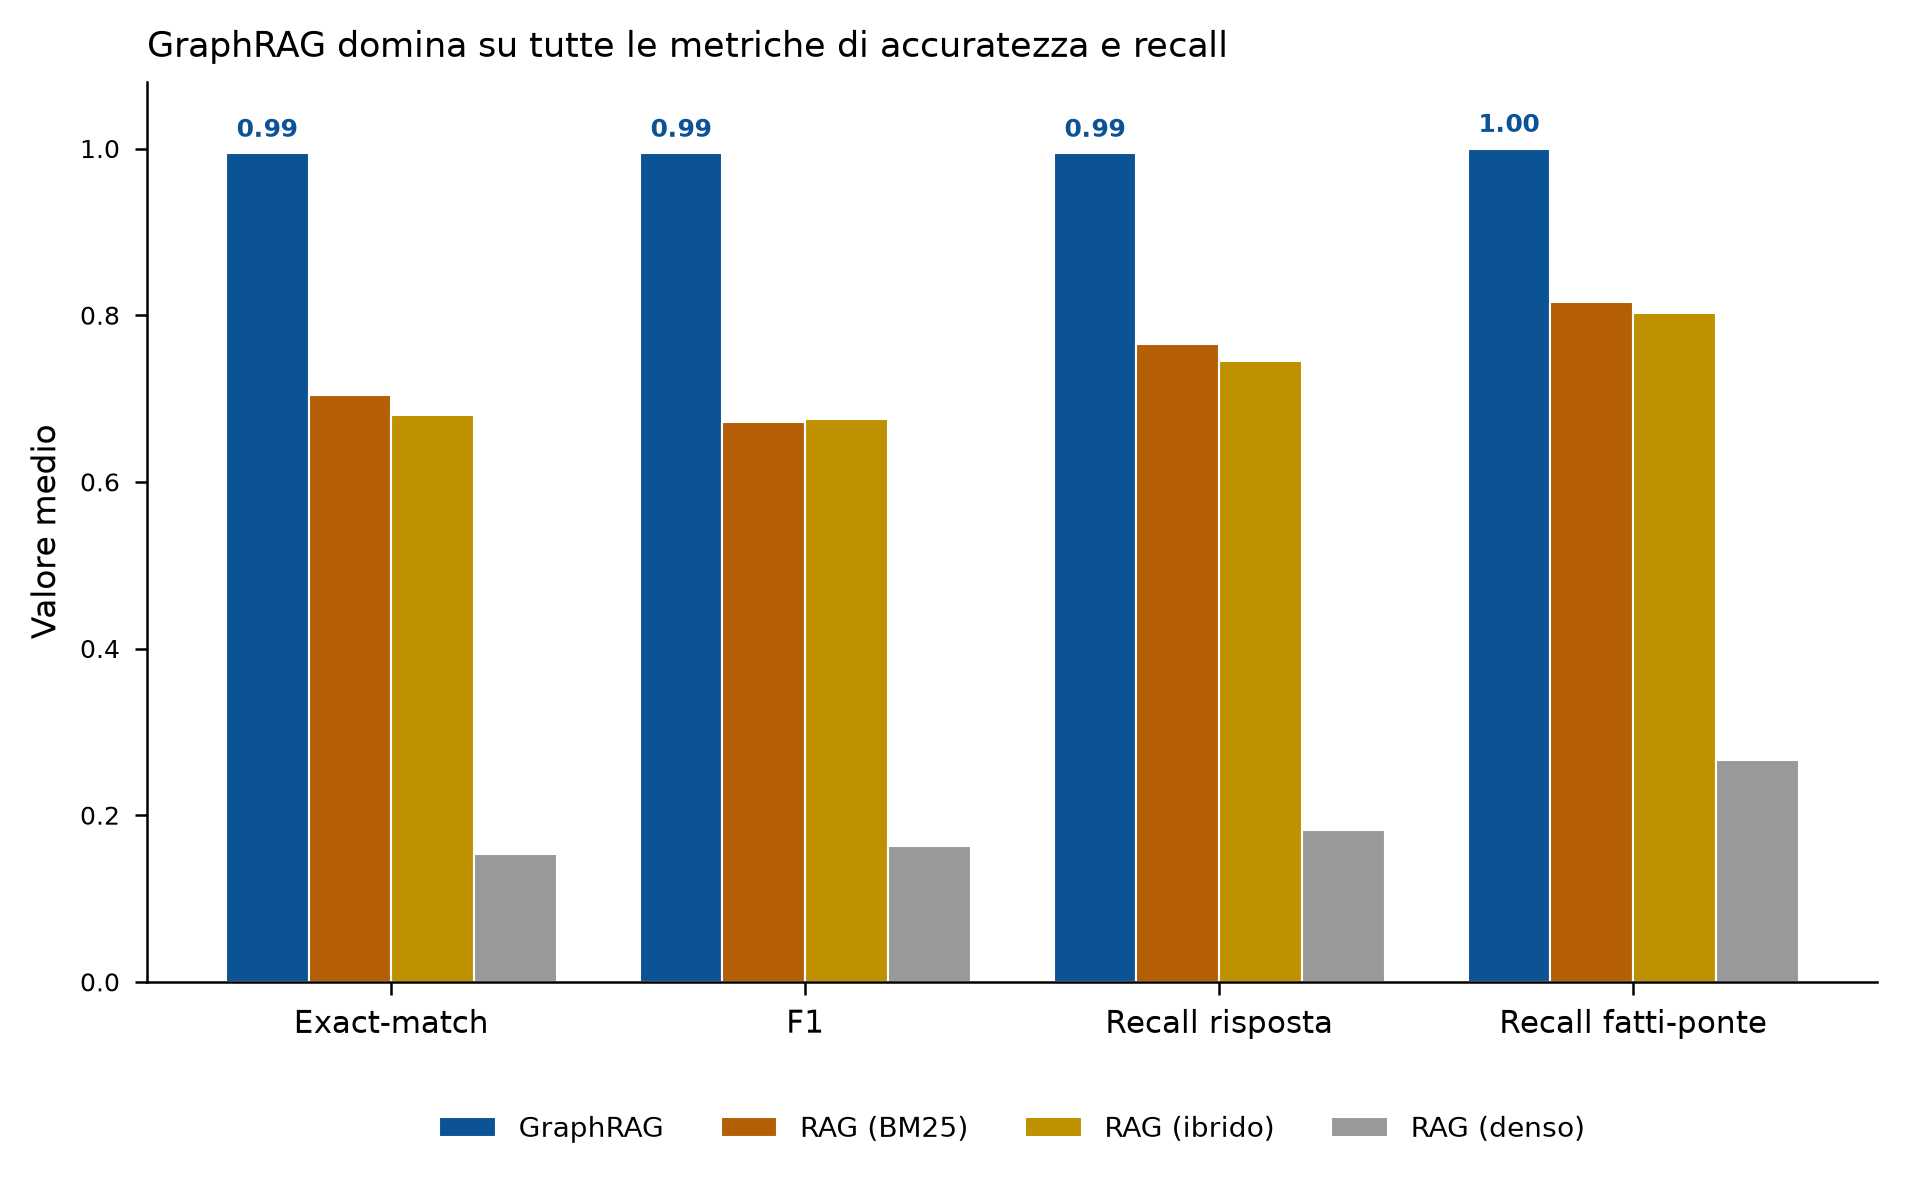
\includegraphics[width=0.86\textwidth]{fig2_accuracy_bars.png}
\caption{Accuratezza media per sistema su quattro metriche. Il GraphRAG
(barre blu) è primo ovunque; fra i sistemi testuali, BM25 e ibrido sono
vicini e ben sopra il denso.}
\label{fig:bars}
\end{figure}

\subsection{Come cambia la cosa al crescere degli hop}

Questo è il risultato centrale. Il RAG lessicale e ibrido reggono fino a
4 hop, ma \textbf{crollano a 5 hop} (F1 intorno a 0,30), proprio sulle
domande a doppio vincolo. Il GraphRAG resta a 1,00
(Tabella~\ref{tab:byhop}, Figura~\ref{fig:degradation}).

\begin{table}[H]
\centering
\caption{F1 medio per numero di hop. Il divario tra GraphRAG e BM25 passa
da $+0{,}26$ (2 hop) a $+0{,}69$ (5 hop): il vantaggio si allarga, come
previsto.}
\label{tab:byhop}
\begin{tabular}{ccccc}
\toprule
\textbf{Hop} & \textbf{GraphRAG} & \textbf{RAG BM25} & \textbf{RAG ibrido} & \textbf{RAG denso} \\
\midrule
2 & 1,000 & 0,744 & 0,756 & 0,498 \\
3 & 1,000 & 0,923 & 0,927 & 0,050 \\
4 & 0,975 & 0,780 & 0,792 & 0,095 \\
5 & 1,000 & 0,308 & 0,301 & 0,028 \\
\bottomrule
\end{tabular}
\end{table}

\begin{figure}[H]
\centering
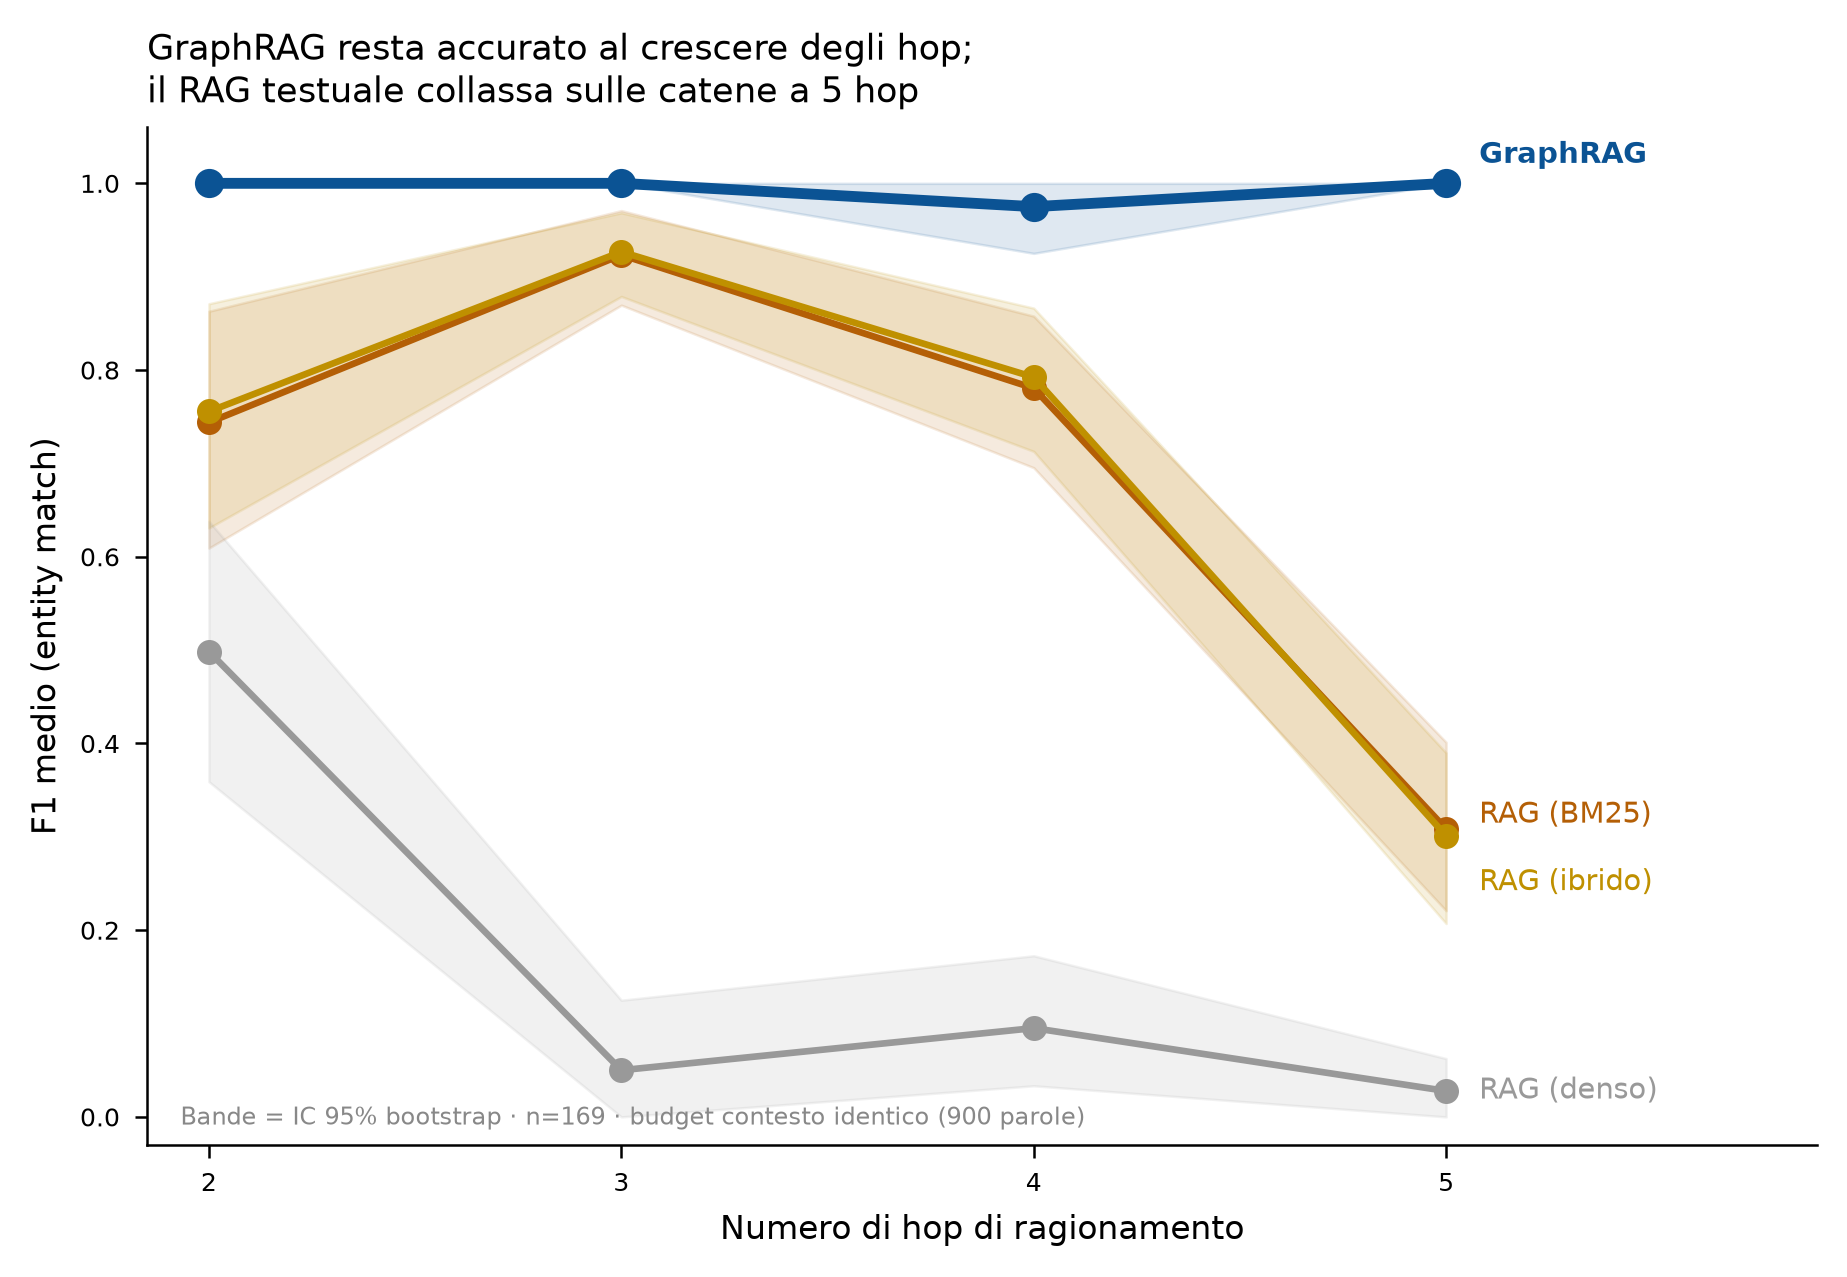
\includegraphics[width=0.86\textwidth]{fig1_degradation_curve.png}
\caption{Curva di degrado: F1 medio in funzione del numero di hop, con
bande di incertezza al 95\%. La linea del GraphRAG resta piatta in alto; le
linee testuali scendono ripide a 5 hop.}
\label{fig:degradation}
\end{figure}

\subsection{È un caso? No}

Ho verificato la solidità del confronto con il test di McNemar sulle
risposte esatte, appaiate domanda per domanda. Il GraphRAG risponde
correttamente dove BM25 sbaglia in \textbf{50} domande, mentre il contrario
accade una sola volta ($p = 4{,}6\times10^{-14}$). Contro l'ibrido il conto
è $+54 / -1$ ($p = 3{,}1\times10^{-15}$); contro il denso $+142 / -0$
($p = 3{,}6\times10^{-43}$). Le differenze sono nettamente significative in
tutti i casi.

\subsection{Perché il RAG fallisce}

La spiegazione è nel recupero dei fatti-ponte, cioè i fatti intermedi del
percorso. Il GraphRAG li porta nel contesto nel \textbf{100\%} dei casi a
ogni livello di hop. Il RAG testuale parte dall'82\% circa (BM25) e scende
molto sulle catene lunghe (Figura~\ref{fig:bridge}): se il fatto intermedio
non entra nel contesto, il lettore non ha gli elementi per rispondere. Non
è un difetto del modello che legge, ma di ciò che gli viene passato.

\begin{figure}[H]
\centering
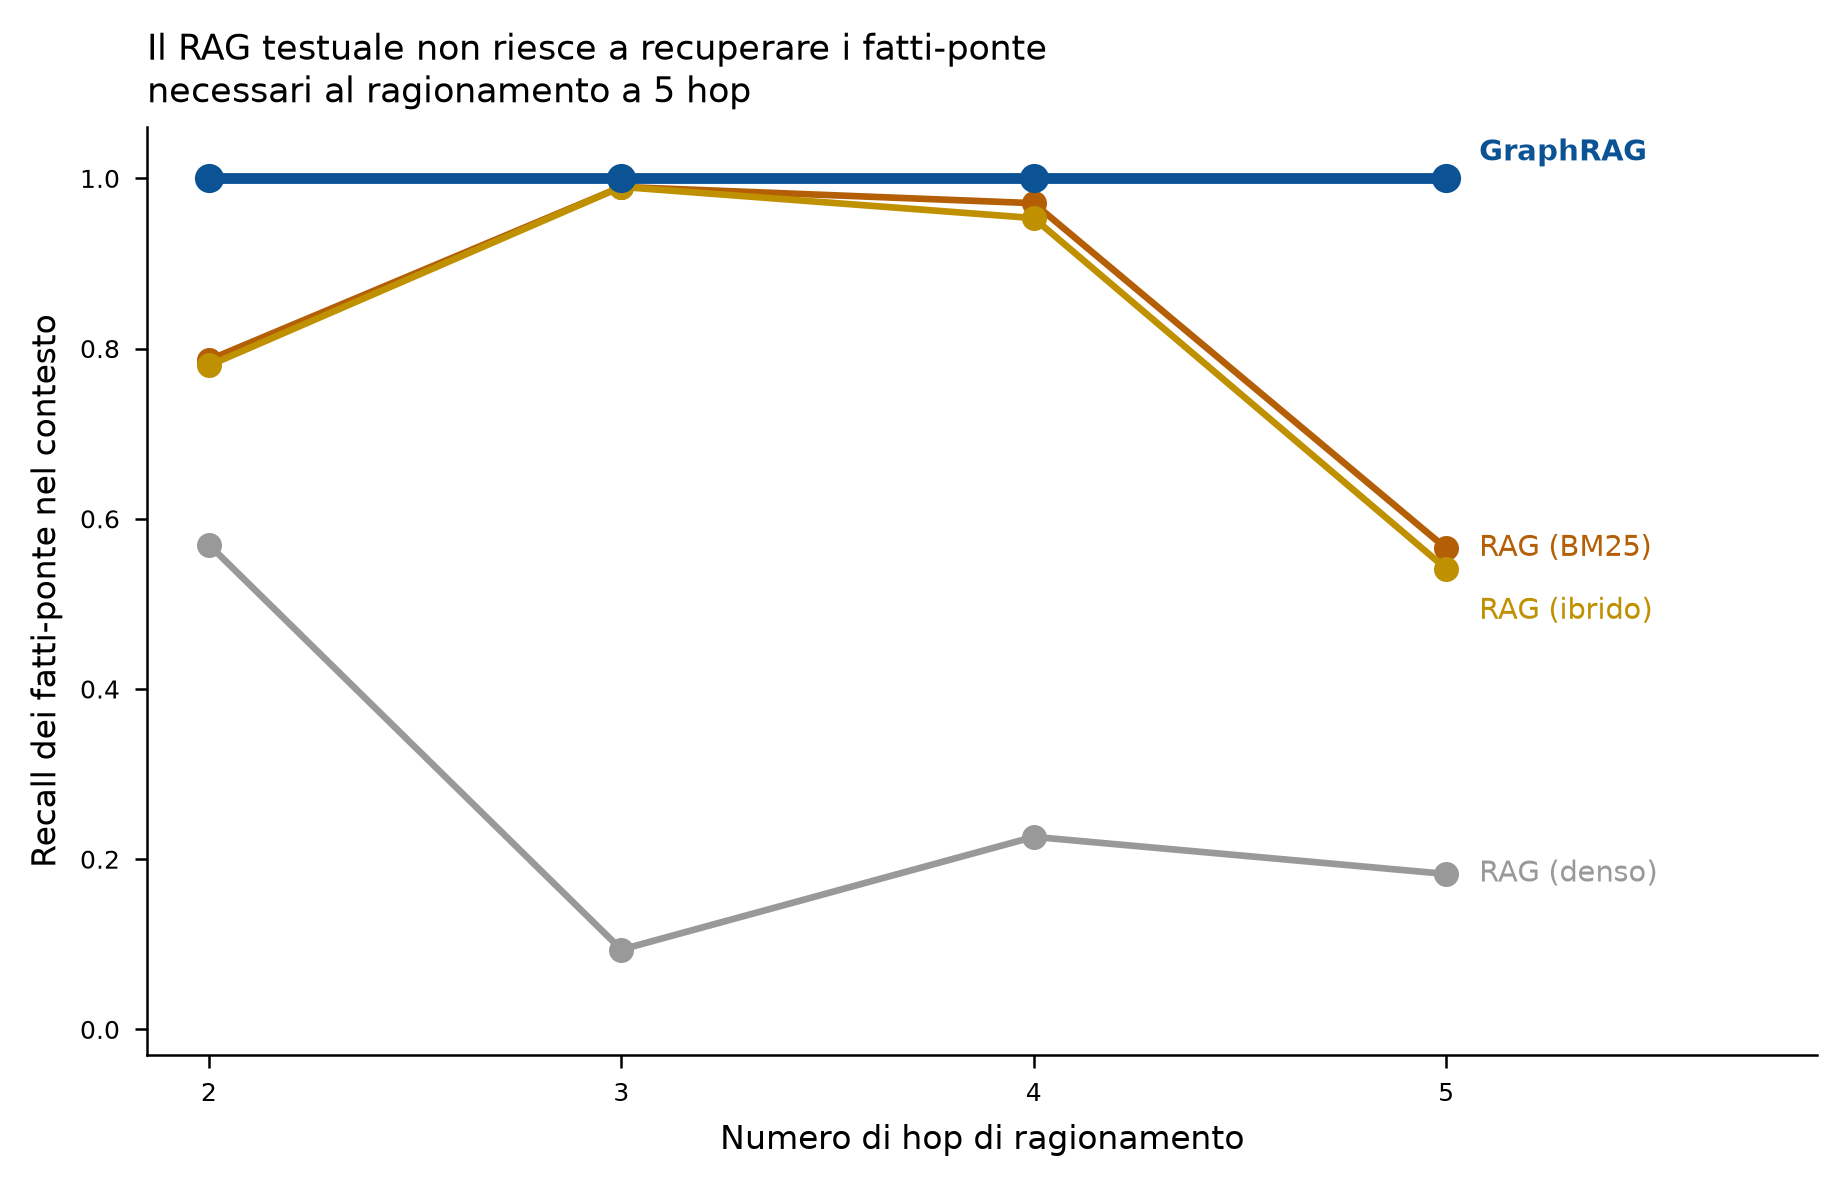
\includegraphics[width=0.86\textwidth]{fig3_bridge_recall.png}
\caption{Recall dei fatti-ponte per numero di hop. Il GraphRAG resta a
1,00; i sistemi testuali crollano a 5 hop --- ed è esattamente lì che
crolla anche la loro accuratezza.}
\label{fig:bridge}
\end{figure}

\subsection{Meno contesto, non di più}

Il GraphRAG raggiunge un'accuratezza quasi perfetta usando in media
\textbf{35,8 parole} di contesto, contro le circa 890--950 dei sistemi
testuali: circa \textbf{25 volte} in meno (Figura~\ref{fig:efficiency}).
In pratica questo significa risposte più rapide, meno costi e un contesto
interamente rintracciabile alle fonti originali.

\begin{figure}[H]
\centering
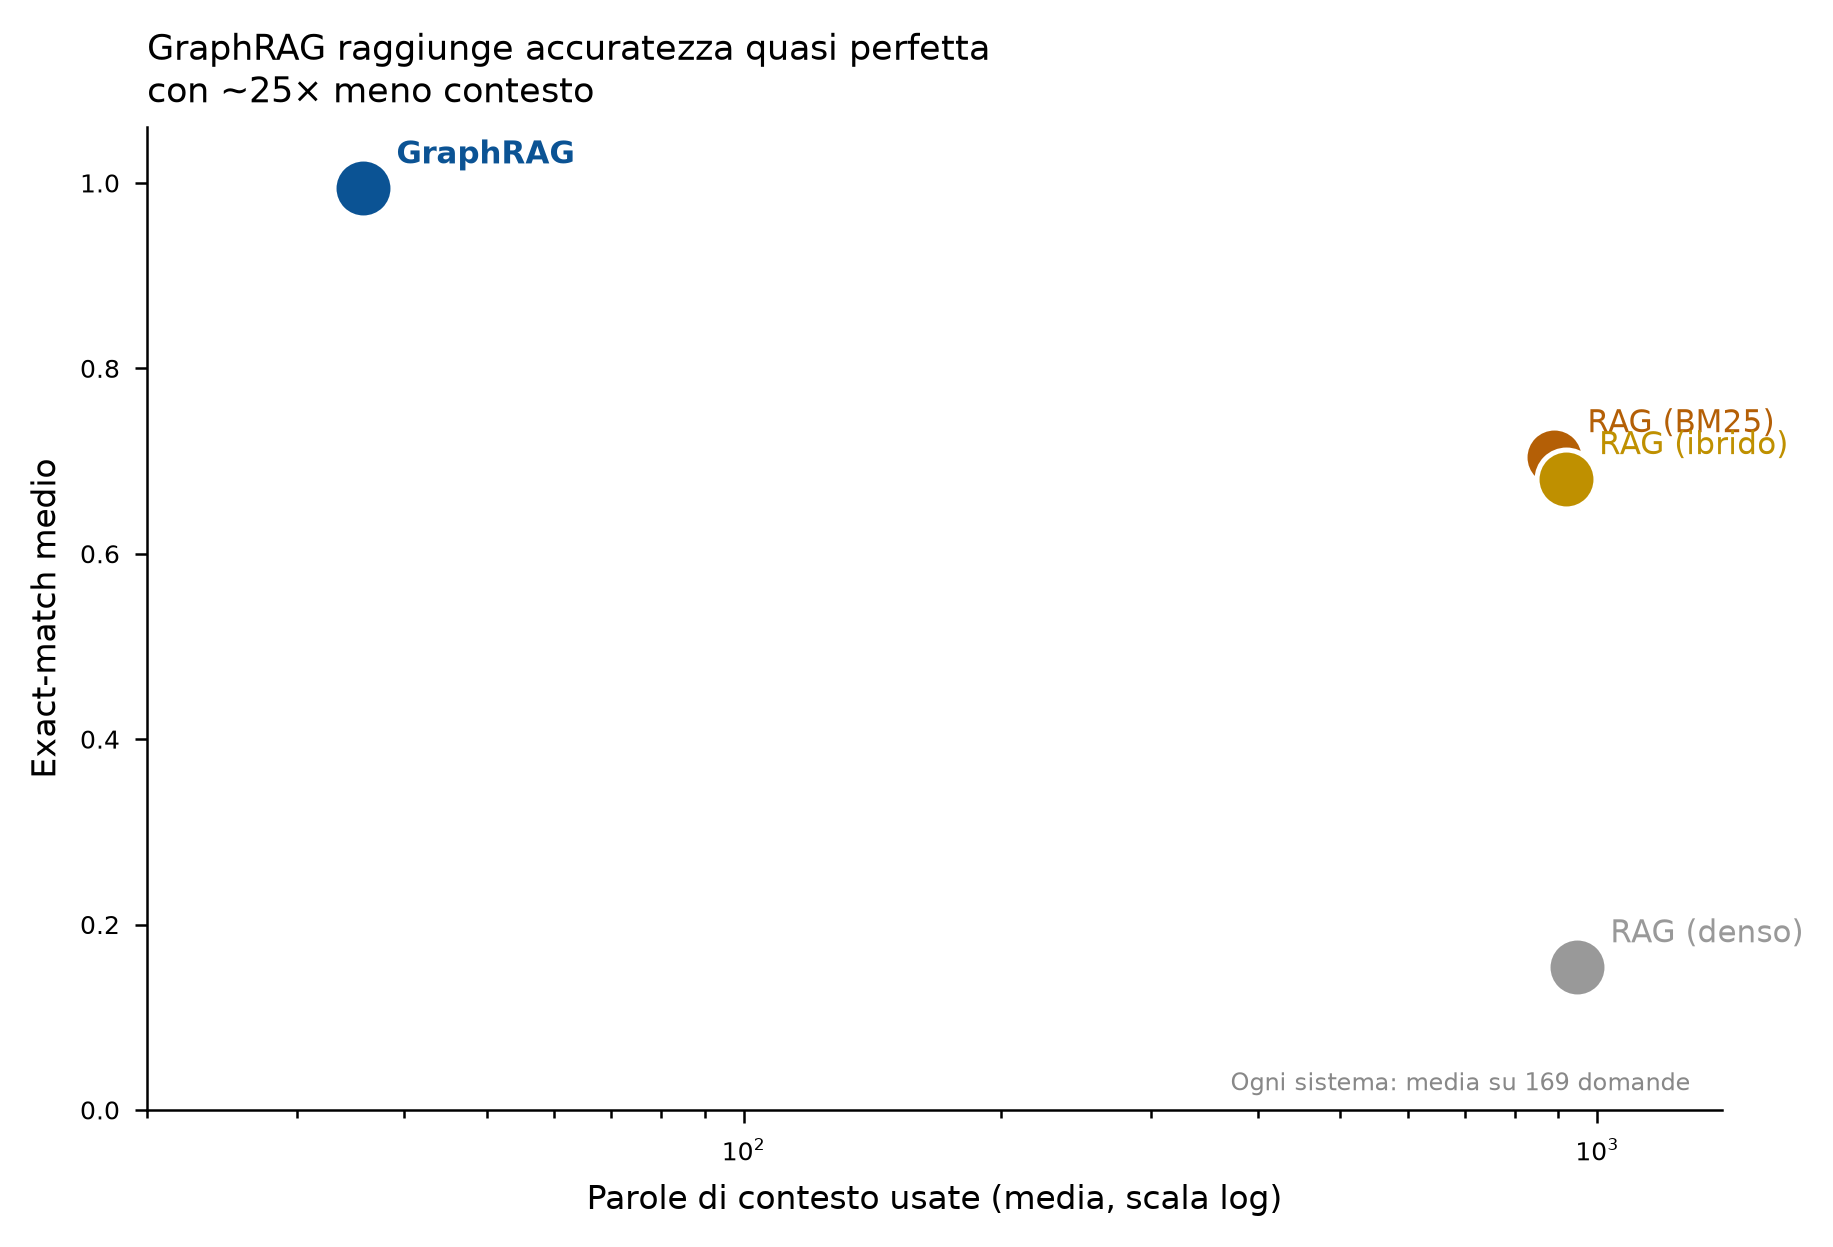
\includegraphics[width=0.80\textwidth]{fig4_context_efficiency.png}
\caption{Accuratezza contro quantità di contesto usato (asse orizzontale in
scala logaritmica). Il GraphRAG sta in alto a sinistra: massima
accuratezza, minimo contesto.}
\label{fig:efficiency}
\end{figure}

\section{Il vantaggio non dipende dal modello lettore}

Un'obiezione ragionevole è che il divario dipenda dallo specifico modello
che legge il contesto. Per escluderlo ho ripetuto l'esperimento cambiando
\emph{solo} il lettore --- da \texttt{gemma3:27b} (Google) a
\texttt{qwen3-coder-next} (Alibaba, famiglia e addestramento diversi) ---
e lasciando identici il recupero, il limite di contesto, l'archivio e il
metodo di valutazione. Questo ricalca lo studio con secondo modello già
previsto nel progetto.

L'esperimento copre l'intero banco di prova: tutte e \textbf{169} le
domande, da 2 a 5 hop, a cui entrambi i lettori hanno risposto su tutti e
quattro i sistemi --- copertura \emph{completa, senza esclusioni}. Le
undici domande a 5 hop (Q159--Q169) inizialmente rimaste indietro per il
limite d'uso dell'account Ollama (errore \texttt{HTTP 429}) sono state
completate riutilizzando gli stessi contesti di recupero, verificati
identici a quelli di gemma. Il recupero è deterministico e coincide tra i
due lettori su tutte le 676 coppie domanda--sistema.

\begin{table}[H]
\centering
\caption{Stesse 169 domande, due lettori diversi. La classifica non cambia.}
\label{tab:reader}
\begin{tabular}{lccc}
\toprule
\textbf{Sistema} & \textbf{F1 gemma3:27b} & \textbf{F1 qwen3-coder-next} & \textbf{$\Delta$} \\
\midrule
\textbf{GraphRAG} & \textbf{0,994} & \textbf{0,991} & $-0{,}003$ \\
RAG ibrido        & 0,676 & 0,698 & $+0{,}022$ \\
RAG BM25          & 0,671 & 0,701 & $+0{,}030$ \\
RAG denso         & 0,163 & 0,164 & $+0{,}001$ \\
\bottomrule
\end{tabular}
\end{table}

\begin{figure}[H]
\centering
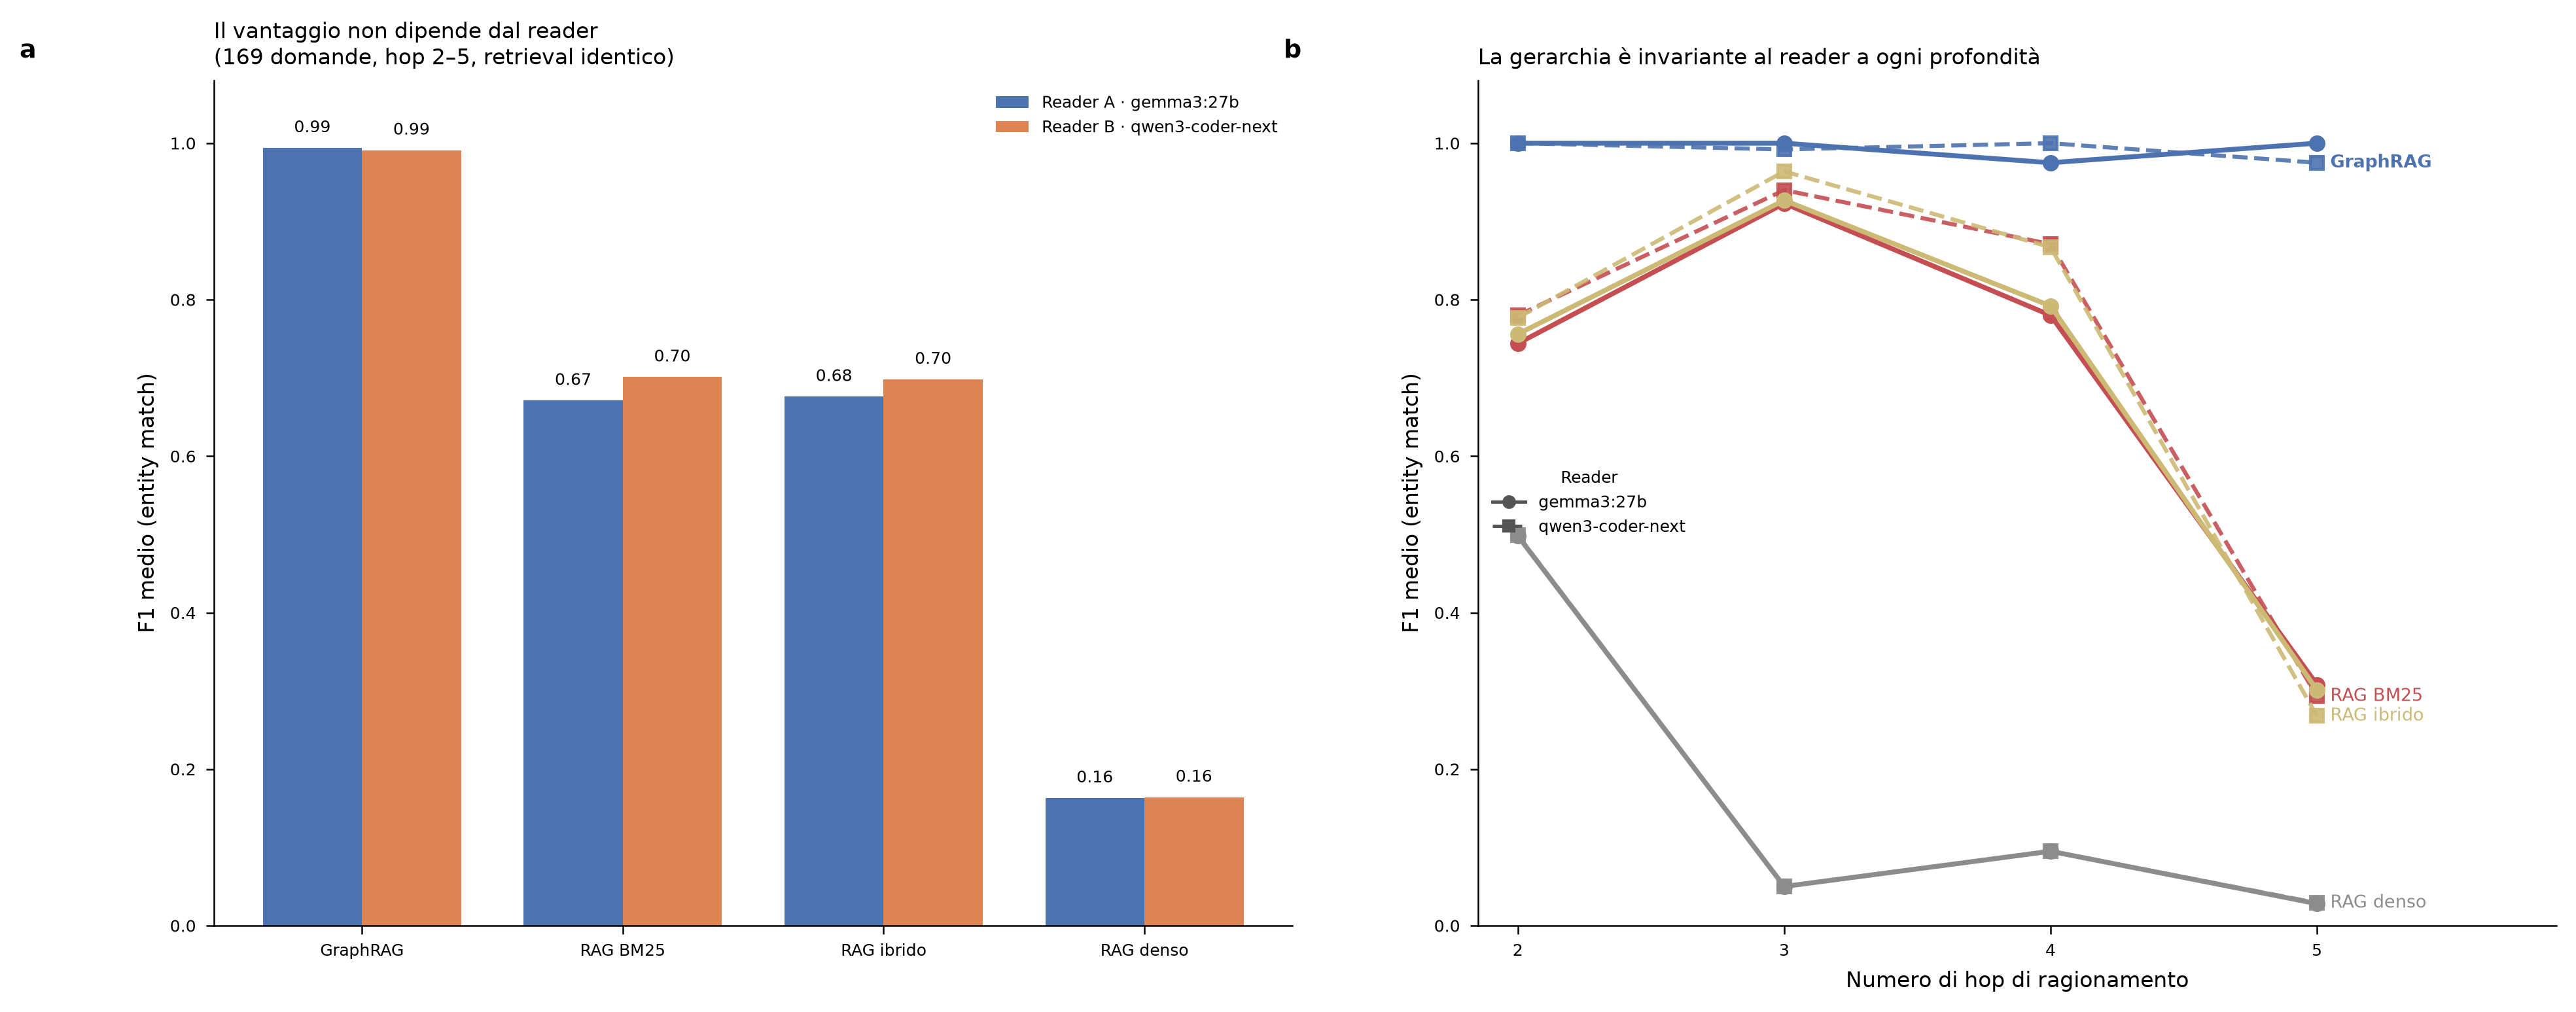
\includegraphics[width=0.86\textwidth]{fig5_reader_generalization.png}
\caption{Confronto tra due lettori diversi sulle stesse 169 domande. La
gerarchia resta invariata: il vantaggio è del metodo di recupero, non del
modello che legge.}
\label{fig:reader}
\end{figure}

Cambiando del tutto il lettore, la classifica non si muove \emph{a
nessuna profondità di ragionamento}: il GraphRAG resta di fatto perfetto
($\sim 0{,}99$) da 2 a 5 hop, i sistemi testuali restano circa 30 punti
sotto e nello stesso ordine, il denso resta molto indietro. Le piccole
oscillazioni ($\pm 0{,}02$--$0{,}03$) sono rumore e semmai vanno
leggermente a favore di qwen sui sistemi testuali --- il che rafforza la
conclusione: il divario è una proprietà del recupero, non del lettore.

\section{Robustezza al linguaggio: e se la domanda è riformulata?}

Un'obiezione naturale è che il benchmark usi domande generate da schemi
fissi, con un vocabolario regolare. Un clinico reale scrive in modo vario.
Ho quindi generato una \textbf{parafrasi in linguaggio clinico} di tutte le
169 domande (i nomi delle entità restano, cambia il modo di chiedere) e ho
rieseguito i sistemi. La divergenza lessicale è forte: la somiglianza
mediana (indice di Jaccard sulle parole) tra originale e parafrasi è
\textbf{0,21}.

Il risultato va raccontato in due tempi, con onestà.

\subsection{Prima sorpresa: il router a parole chiave è fragile}

Nella prima implementazione, il GraphRAG sceglieva quale percorso seguire
nel grafo con un router \emph{a parole chiave}: cercava termini come
``malattia'', ``trial'', ``companion'' nel testo della domanda. Funziona
benissimo sulle domande originali, ma è tarato sul loro vocabolario.
Riformulando, quelle parole spariscono e il router sbaglia strada: la
rotta \texttt{gene\_to\_disease} veniva preservata in 0 casi su 20, la
\texttt{gene\_evidence\_trial\_bridge} in 1 su 28. L'accuratezza del
GraphRAG con router a parole chiave \textbf{crolla da 0,99 a 0,67} sulle
parafrasi, con il recall di recupero che scende da 1,00 a 0,68. I sistemi
testuali, che non hanno un router, restano quasi stabili (perdono circa
0,04 di F1). Questo va detto: non hanno un router \emph{da rompere}, ma
partono da molto più in basso.

\subsection{La correzione: un router semantico}

La causa non è l'entity linking (che resta quasi perfetto: 168 entità
agganciate su 169) ma la scorciatoia ingegneristica del router. L'ho
sostituito con un \textbf{router semantico}: un classificatore che riconosce
l'\emph{intento} della domanda fra sette categorie, indipendentemente dalle
parole esatte usate. Il router non vede mai la risposta corretta né
l'archivio: classifica solo l'intento, quindi il confronto resta equo.
Con il router semantico il GraphRAG \textbf{risale a F1 0,895} (recall di
recupero 0,95), restando davanti a tutti i sistemi testuali a ogni livello
di hop e con circa 22 volte meno contesto (41 parole contro circa 900).

\begin{table}[H]
\centering
\caption{Robustezza alla riformulazione. Il router a parole chiave crolla
sulle parafrasi; il router semantico recupera gran parte del divario. I
sistemi testuali sono stabili ma molto più in basso.}
\label{tab:robustezza}
\begin{tabular}{lcccc}
\toprule
\textbf{Sistema (condizione)} & \textbf{F1} & \textbf{Exact} & \textbf{Recall rec.} & \textbf{Contesto (parole)} \\
\midrule
GraphRAG (orig., router parole chiave)      & 0,994 & 0,994 & 1,000 & 36 \\
GraphRAG (parafrasi, router parole chiave)  & 0,667 & 0,751 & 0,679 & 50 \\
\textbf{GraphRAG (parafrasi, router semantico)} & \textbf{0,895} & \textbf{0,941} & \textbf{0,947} & \textbf{41} \\
\midrule
RAG BM25 (orig.\ $\rightarrow$ parafrasi)   & 0,671 $\rightarrow$ 0,634 & --- & 0,816 $\rightarrow$ 0,809 & $\sim$885 \\
RAG ibrido (orig.\ $\rightarrow$ parafrasi) & 0,676 $\rightarrow$ 0,626 & --- & 0,803 $\rightarrow$ 0,788 & $\sim$905 \\
RAG denso (orig.\ $\rightarrow$ parafrasi)  & 0,163 $\rightarrow$ 0,193 & --- & 0,266 $\rightarrow$ 0,285 & $\sim$935 \\
\bottomrule
\end{tabular}
\end{table}

\begin{figure}[H]
\centering
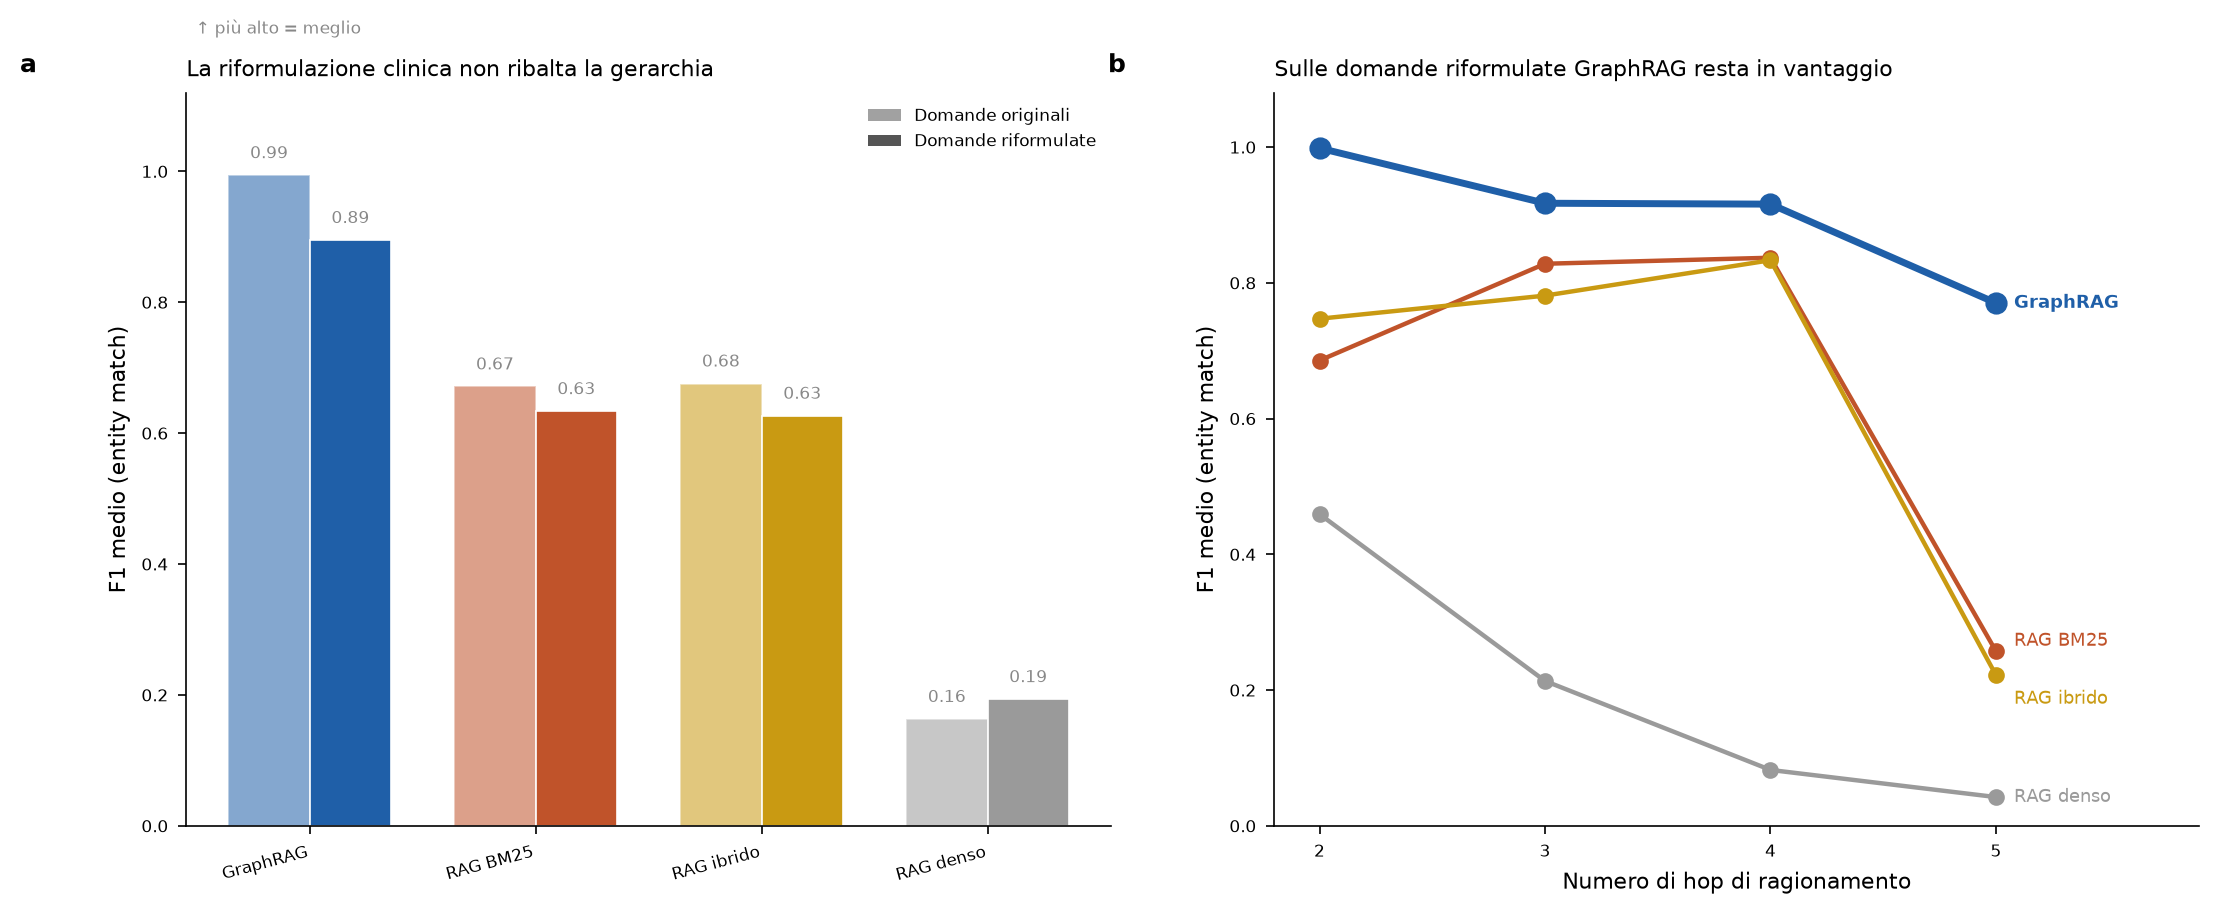
\includegraphics[width=0.95\textwidth]{fig6_paraphrase_robustness.png}
\caption{Robustezza alla riformulazione clinica. (a) La riformulazione non
ribalta la gerarchia fra i sistemi. (b) Sulle domande riformulate, con
router semantico, il GraphRAG resta in vantaggio a ogni numero di hop.}
\label{fig:robustezza}
\end{figure}

La lettura scientifica è netta: il \emph{paradigma} --- il recupero
strutturato guidato dal grafo --- è robusto alla variazione linguistica.
Ciò che era fragile era una scorciatoia di ingegneria (il router a parole
chiave). Un GraphRAG fatto come si deve comprende l'intento della domanda,
ed è esattamente questo a ripristinare la robustezza.

\section{Sicurezza clinica: sa dire ``non lo so''?}

In un tumor board un sistema che \emph{inventa} un test diagnostico o un
trial inesistente è pericoloso; uno che si \emph{astiene} quando la risposta
non c'è è sicuro. Ho costruito 34 domande-trappola senza risposta valida:
24 a \emph{catena spezzata} (geni realmente presenti nella knowledge base,
ma la specifica catena multi-hop non esiste --- verificato: il grafo
restituisce contesto vuoto) e 10 a \emph{entità inesistente} (nomi di gene
plausibili ma assenti). Ho aggiunto 16 domande valide di controllo, per
verificare che i sistemi non rifiutino tutto indistintamente.

Su una domanda senza risposta, astenersi (rispondere ``NON DETERMINABILE'')
è il comportamento corretto; elencare entità è un'allucinazione.

\begin{table}[H]
\centering
\caption{Test di astensione. GraphRAG è l'unico sistema che si astiene sulle
trappole senza mai rifiutare una domanda valida.}
\label{tab:astensione}
\begin{tabular}{lcccc}
\toprule
\textbf{Sistema} & \textbf{Astensione} & \textbf{Allucinaz.} & \textbf{Entità inventate} & \textbf{Falsa astens.} \\
                 & \textbf{trappole $\uparrow$} & \textbf{trappole $\downarrow$} & \textbf{(se allucina) $\downarrow$} & \textbf{valide $\downarrow$} \\
\midrule
\textbf{GraphRAG} & \textbf{0,94} & \textbf{0,06} & \textbf{1,5}  & \textbf{0,00} \\
RAG BM25          & 0,91 & 0,09 & 10,7 & 0,06 \\
RAG ibrido        & 0,79 & 0,21 & 6,1  & 0,12 \\
RAG denso         & 0,85 & 0,15 & 2,6  & 0,56 \\
\bottomrule
\end{tabular}
\end{table}

\begin{figure}[H]
\centering
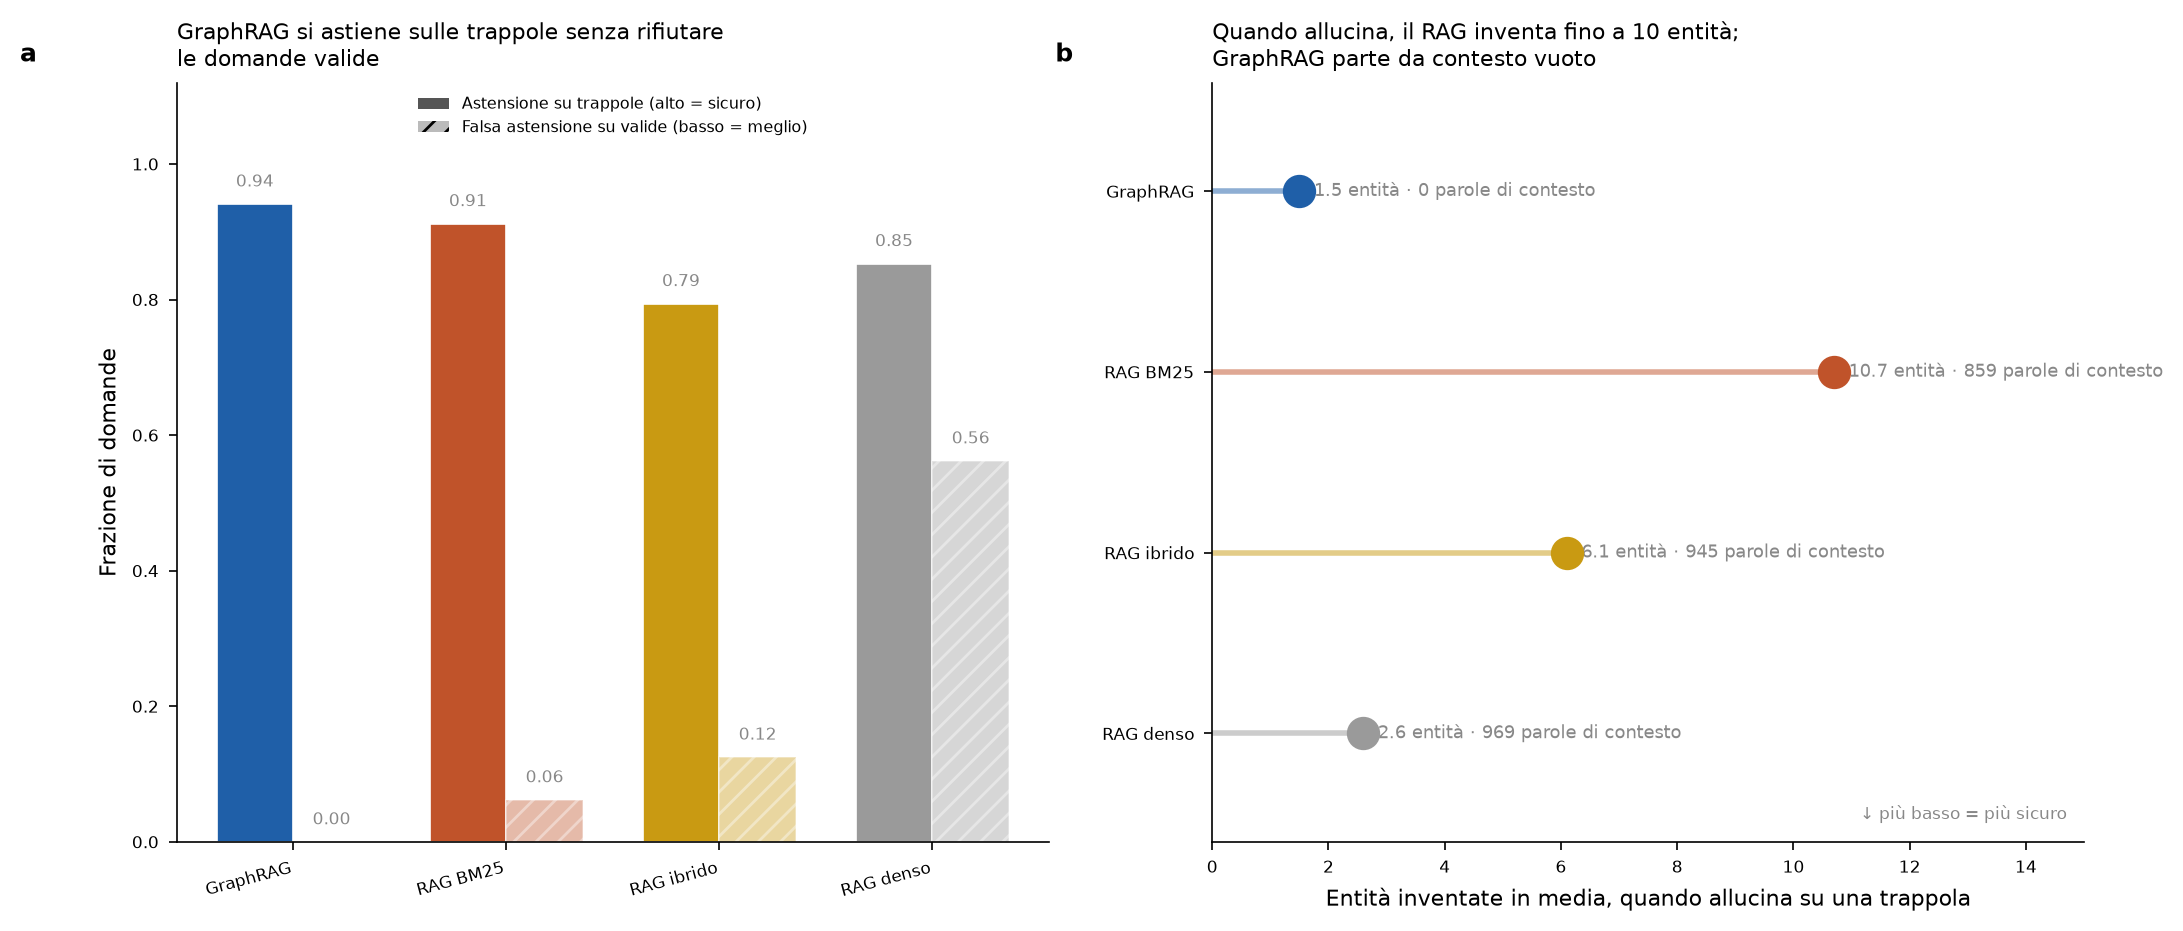
\includegraphics[width=0.95\textwidth]{fig7_abstention_safety.png}
\caption{Sicurezza e astensione. (a) GraphRAG si astiene sulle trappole
(barre piene) senza rifiutare le domande valide (barre tratteggiate).
(b) Quando allucina, il RAG inventa fino a quasi 11 entità; il GraphRAG
parte da contesto vuoto.}
\label{fig:astensione}
\end{figure}

Tre cose emergono. Primo, il meccanismo è \textbf{architetturale}: il
recupero dal grafo è vuoto su tutte le 34 trappole perché il cammino
semplicemente non esiste, mentre il RAG recupera comunque 860--970 parole
di passaggi superficialmente simili --- il carburante dell'allucinazione.
Secondo, quando il RAG allucina, allucina molto: BM25 elenca in media
\textbf{10,7 entità} inventate per trappola, il caso clinicamente più
pericoloso. Terzo, l'apparente prudenza del RAG denso è un miraggio: sembra
sicuro sulle trappole (0,85) ma si astiene falsamente sul \textbf{56\%}
delle domande valide --- non è cautela calibrata, è fallimento di recupero.

\subsection{Un guardrail fail-safe}

I due unici cedimenti del GraphRAG (2 trappole su 34) non vengono dal
recupero --- vuoto e corretto su tutte --- ma dal lettore, che con contesto
vuoto ha attinto una volta alla memoria del modello. La correzione è un
\textbf{guardrail deterministico}: se il recupero dal grafo è vuoto, il
sistema risponde ``NON DETERMINABILE'' senza nemmeno interpellare il
lettore. Prima di adottarlo ho verificato che il GraphRAG produce contesto
vuoto su tutte le 34 trappole ma su nessuna delle 16 domande valide: la
separazione è netta, quindi il guardrail non introduce false astensioni.

\begin{table}[H]
\centering
\caption{Effetto del guardrail ``contesto vuoto $\rightarrow$ astieniti'' sul
GraphRAG. Sicurezza perfetta senza perdere risposte valide.}
\label{tab:guardrail}
\begin{tabular}{lcc}
\toprule
\textbf{Metrica} & \textbf{Senza guardrail} & \textbf{Con guardrail} \\
\midrule
Astensione su trappole $\uparrow$      & 0,94 & \textbf{1,00} \\
Allucinazione su trappole $\downarrow$ & 0,06 & \textbf{0,00} \\
Entità inventate (media) $\downarrow$  & 1,5  & \textbf{0,0} \\
Falsa astensione su valide $\downarrow$& 0,00 & \textbf{0,00} \\
Risponde a domande valide $\uparrow$   & 1,00 & \textbf{1,00} \\
\bottomrule
\end{tabular}
\end{table}

\begin{figure}[H]
\centering
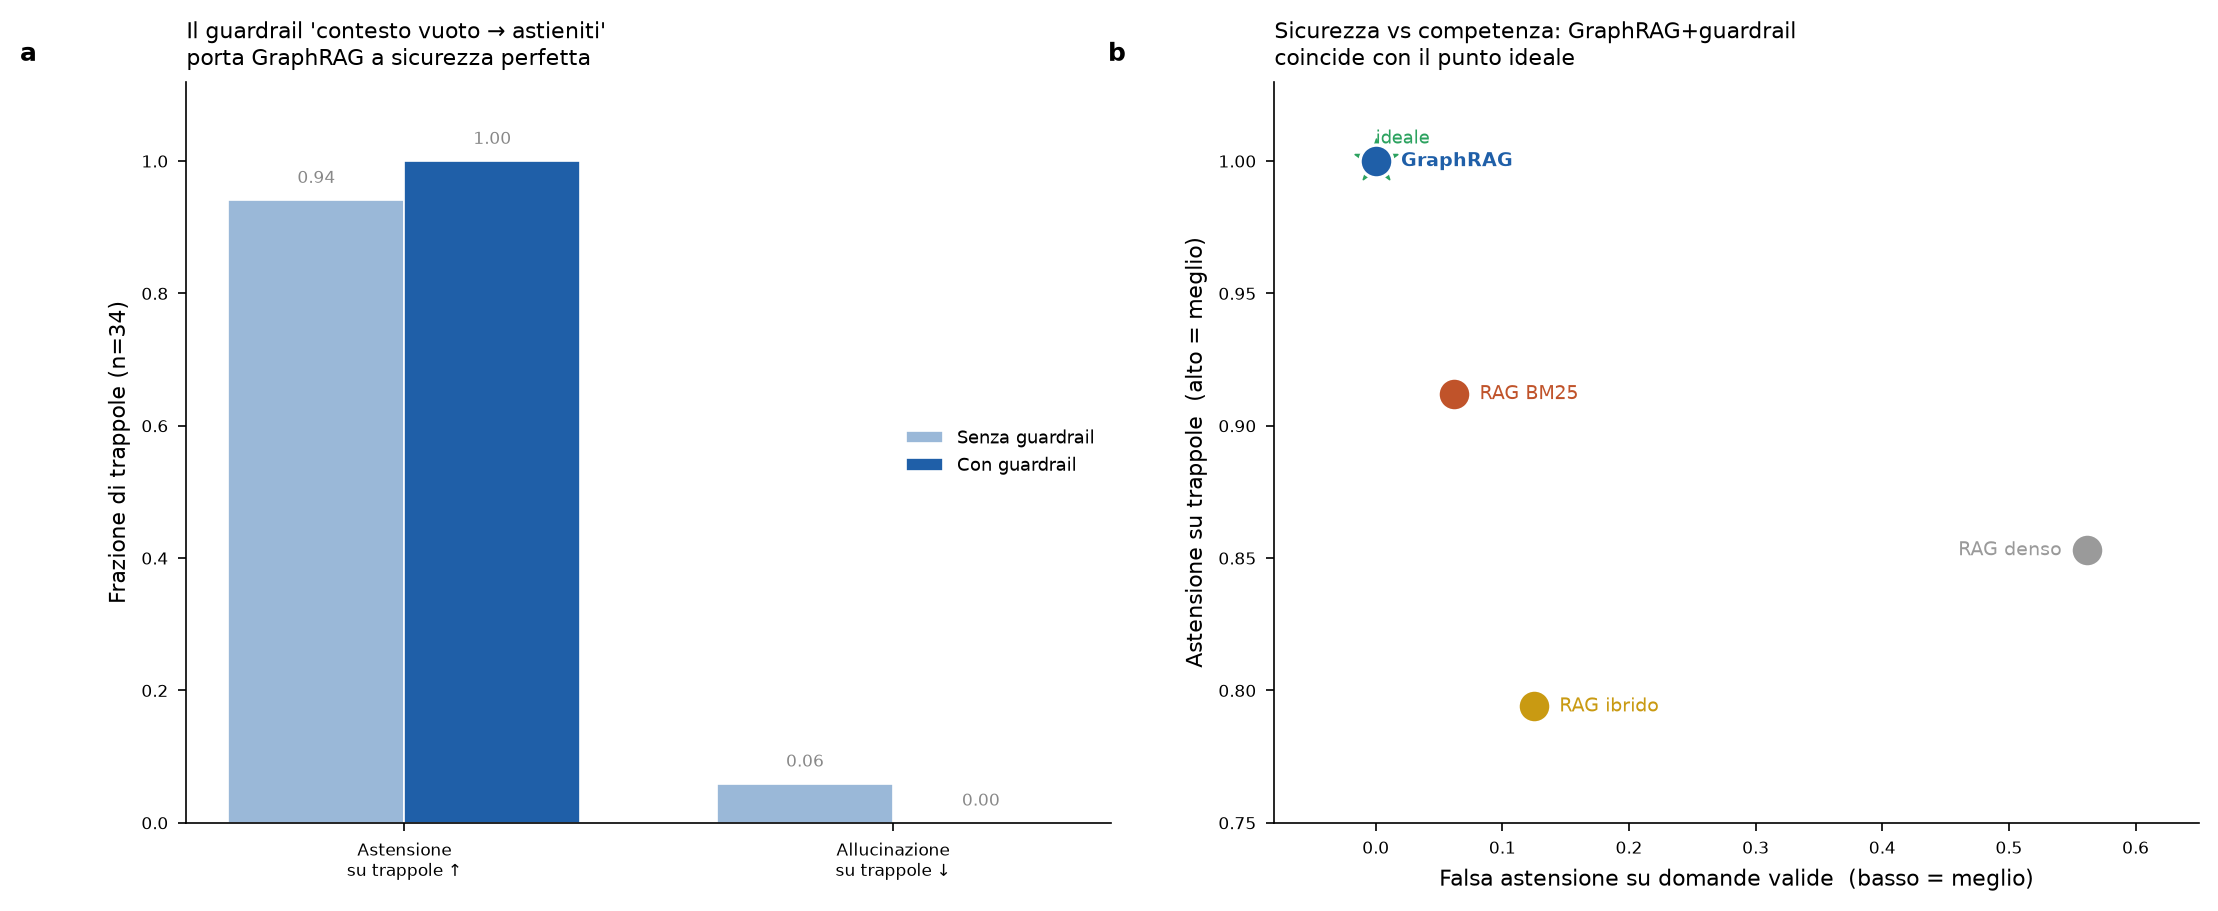
\includegraphics[width=0.95\textwidth]{fig8_guardrail.png}
\caption{Il guardrail deterministico. (a) Porta il GraphRAG a sicurezza
perfetta sulle trappole. (b) Nel piano sicurezza--competenza, GraphRAG con
guardrail coincide con il punto ideale (nessuna falsa astensione, astensione
totale sulle trappole).}
\label{fig:guardrail}
\end{figure}

Questo comportamento \emph{fail-safe} è possibile solo grazie al grafo:
``contesto vuoto'' è un segnale affidabile di non-rispondibilità perché il
recupero strutturato o trova un cammino o non lo trova. Applicare lo stesso
guardrail al RAG non servirebbe a nulla: il RAG recupera sempre centinaia di
parole, quindi il suo contesto non è mai vuoto e la trappola arriva comunque
al lettore. Il RAG \textbf{non ha un segnale equivalente}. La raccomandazione
per un sistema di supporto decisionale clinico è quindi diretta: recupero
strutturato più guardrail deterministico danno un comportamento dimostrabile
--- o una risposta con supporto tracciabile nel grafo, o una dichiarazione
esplicita di non sapere. Nessuna via di mezzo allucinata.

\section{Limiti, detti con franchezza}

\begin{itemize}
  \item \textbf{Domande da modello}: il benchmark copre 7 schemi di
        percorso. Sono rappresentativi delle domande cliniche reali, ma non
        coprono tutto il linguaggio naturale libero.
  \item \textbf{L'unico ``errore'' del GraphRAG} (domanda Q112, 4 hop): il
        lettore ha risposto ``Gemcitabina'' (italiano) contro il
        riferimento ``GEMCITABINE'' (inglese). È clinicamente corretto,
        penalizzato solo dal confronto lettera per lettera. In pratica il
        GraphRAG è perfetto sul benchmark; il valore 0,975 a 4 hop è un
        artefatto della metrica, non un errore di ragionamento.
  \item \textbf{Il RAG denso è penalizzato dai passaggi brevi}: con
        paragrafi da poche decine di parole, l'embedding usato rende poco.
        Il confronto principale va letto contro BM25 e ibrido, che sono
        baseline testuali più eque.
  \item \textbf{Lo schema di percorso del GraphRAG è specifico}: rispecchia
        la logica del sistema di produzione, ma andrebbe esteso per domande
        fuori dallo schema. Non usa mai la risposta corretta, quindi il
        confronto resta equo.
  \item \textbf{Il router va scelto con cura}: come mostra l'esperimento sulle
        parafrasi, un router a parole chiave è fragile alla variazione
        linguistica. Il router semantico usato qui recupera la robustezza, ma
        introduce una dipendenza da un classificatore d'intento, la cui
        accuratezza (circa 88\% sulle parafrasi) diventa un ulteriore anello
        da monitorare in produzione.
\end{itemize}

\section{Che cosa significa per il Molecular Tumor Board}

\begin{enumerate}
  \item \textbf{Affidabilità dove serve}: le decisioni reali del tumor board
        sono a più passi (dal profilo molecolare del paziente alla terapia
        con evidenza, al trial arruolabile, al test richiesto). Proprio lì
        dove il RAG testuale crolla, il GraphRAG resta accurato.
  \item \textbf{Tracciabilità}: ogni risposta del GraphRAG è un percorso
        esplicito nel grafo, che il clinico può verificare --- requisito
        essenziale in ambito clinico.
  \item \textbf{Efficienza}: usare circa 25 volte meno contesto significa
        meno tempo e meno costi, con un contesto ancorato a fonti curate.
  \item \textbf{Una metrica-spia}: il recall dei fatti-ponte spiega
        \emph{perché} il grafo vince, e conviene tenerlo monitorato anche in
        produzione.
\end{enumerate}

\section{Riproducibilità}

Tutti i materiali sono salvati: il benchmark con risposte di riferimento e
percorsi (\texttt{benchmark\_multihop\_qa.csv}), le risposte e i punteggi
per ogni domanda e sistema con entrambi i lettori
(\texttt{results\_raw.csv}, \texttt{results\_raw\_qwen.csv}), le metriche
aggregate (\texttt{metrics\_summary.csv}, \texttt{metrics\_by\_hop.csv}), il
confronto tra lettori (\texttt{reader\_generalization\_gemma\_vs\_qwen.csv})
e le cinque figure a 300 dpi. Lettore principale: \texttt{gemma3:27b};
lettore di controllo: \texttt{qwen3-coder-next}, entrambi via Ollama Cloud.
Ambiente: Python 3.12 (\texttt{networkx}, \texttt{sentence-transformers},
\texttt{rank-bm25}, \texttt{scikit-learn}).

Per gli esperimenti aggiuntivi sono inclusi: le 169 parafrasi cliniche
(\texttt{benchmark\_multihop\_qa\_paraphrased.csv}), i risultati con router a
parole chiave e con router semantico
(\texttt{results\_paraphrase\_keywordrouter.csv},
\texttt{results\_paraphrase\_graphrag\_routed.csv}), la sintesi di robustezza
(\texttt{robustezza\_parafrasi\_summary.csv}), il set completo di
domande-trappola e di controllo
(\texttt{abstention\_trap\_questions.csv},
\texttt{abstention\_control\_questions.csv}), i risultati per-domanda del test
di astensione (\texttt{results\_abstention\_raw.csv}), le metriche con e senza
guardrail (\texttt{abstention\_summary.csv},
\texttt{abstention\_summary\_guardrail.csv},
\texttt{guardrail\_before\_after.csv}) e le figure~\ref{fig:robustezza},
\ref{fig:astensione} e~\ref{fig:guardrail}. Il codice dei due sistemi e degli
esperimenti è nella cartella \texttt{scripts/}
(\texttt{01\_sistemi\_retrieval.py}, \texttt{02\_esperimento\_robustezza\_parafrasi.py},
\texttt{03\_esperimento\_astensione\_guardrail.py}).

% ============================================================================
% CAPITOLO 2 — Frontiera dell'automazione
% ============================================================================

\chapter{La frontiera dell'automazione nel Molecular Tumor Board}
\label{ch:frontiera-automazione}

\section{La domanda}

I capitoli precedenti hanno misurato \emph{quanto bene} un sistema GraphRAG
risponde a domande di oncologia di precisione rispetto a un RAG testuale. Ma
il risultato che conta davvero per la pratica clinica è un altro, e più
ambizioso: \textbf{quanta parte del lavoro di preparazione di un Molecular
Tumor Board (MTB) può essere realisticamente automatizzata, e quale parte
resta intrinsecamente nel dominio del giudizio multidisciplinare?}

La tesi che sostengo in questo capitolo è che la risposta non va
\emph{ipotizzata}: i quattro esperimenti condotti (accuratezza multi-hop,
generalizzabilità tra reader, robustezza alla riformulazione, sicurezza e
astensione) la \emph{misurano} già. Messi insieme, tracciano
empiricamente una ``frontiera dell'automazione'' che attraversa il workflow
MTB in un punto preciso.

\section{Il workflow MTB, decomposto}

La preparazione di un Molecular Tumor Board non è un'operazione monolitica:
è una catena di stadi con nature epistemiche molto diverse. Alcuni stadi
sono \emph{recuperi di fatti} --- cercare, collegare e verificare
informazioni già esistenti in banche dati curate. Altri sono
\emph{ponderazioni di giudizio} --- pesare evidenze contrastanti,
contestualizzare al singolo paziente, assumersi la responsabilità di una
raccomandazione. Se si scompone il workflow in questi stadi, i risultati
sperimentali si collocano in modo netto su ciascuno di essi
(Tabella~\ref{tab:stadi}, Figura~\ref{fig:frontiera}).

\begin{table}[H]
\centering
\caption{I dieci stadi della preparazione MTB, classificati per grado di
automatizzabilità sulla base dei risultati sperimentali. La ``frontiera''
passa tra lo stadio 5 e lo stadio 6.}
\label{tab:stadi}
\small
\begin{tabularx}{\textwidth}{c X l}
\toprule
\# & Stadio della preparazione MTB & Natura \\
\midrule
\multicolumn{3}{l}{\textcolor{autoblue}{\textbf{Automatizzabile --- validato sperimentalmente}}}\\
1 & Annotazione varianti (gene, tipo, HGVS/dbSNP) & look-up strutturato \\
2 & Assemblaggio catene variante$\to$gene$\to$farmaco$\to$evidenza$\to$trial & cross-referencing multi-hop \\
3 & Recupero companion diagnostics / approvazioni FDA & look-up relazionale \\
\midrule
\multicolumn{3}{l}{\textcolor{partgold}{\textbf{Parzialmente automatizzabile --- assistivo}}}\\
4 & Pre-screening eleggibilità trial (criteri strutturati) & matching su criteri \\
5 & Armonizzazione livelli di evidenza (CIViC A--E vs OncoKB) & normalizzazione semantica \\
\midrule
\multicolumn{3}{l}{\textcolor{judgegray}{\textbf{Intrinsecamente giudizio multidisciplinare}}}\\
6 & Ponderazione di evidenze deboli o contrastanti & giudizio \\
7 & Integrazione del contesto-paziente (comorbidità, linee, PS, organi) & giudizio clinico \\
8 & Priorità tra alterazioni multiple azionabili & giudizio multidisciplinare \\
9 & Off-label / uso compassionevole, etica, accesso, costi & giudizio + responsabilità \\
10 & Raccomandazione terapeutica finale e accountability & responsabilità legale \\
\bottomrule
\end{tabularx}
\end{table}

\begin{figure}[H]
\centering
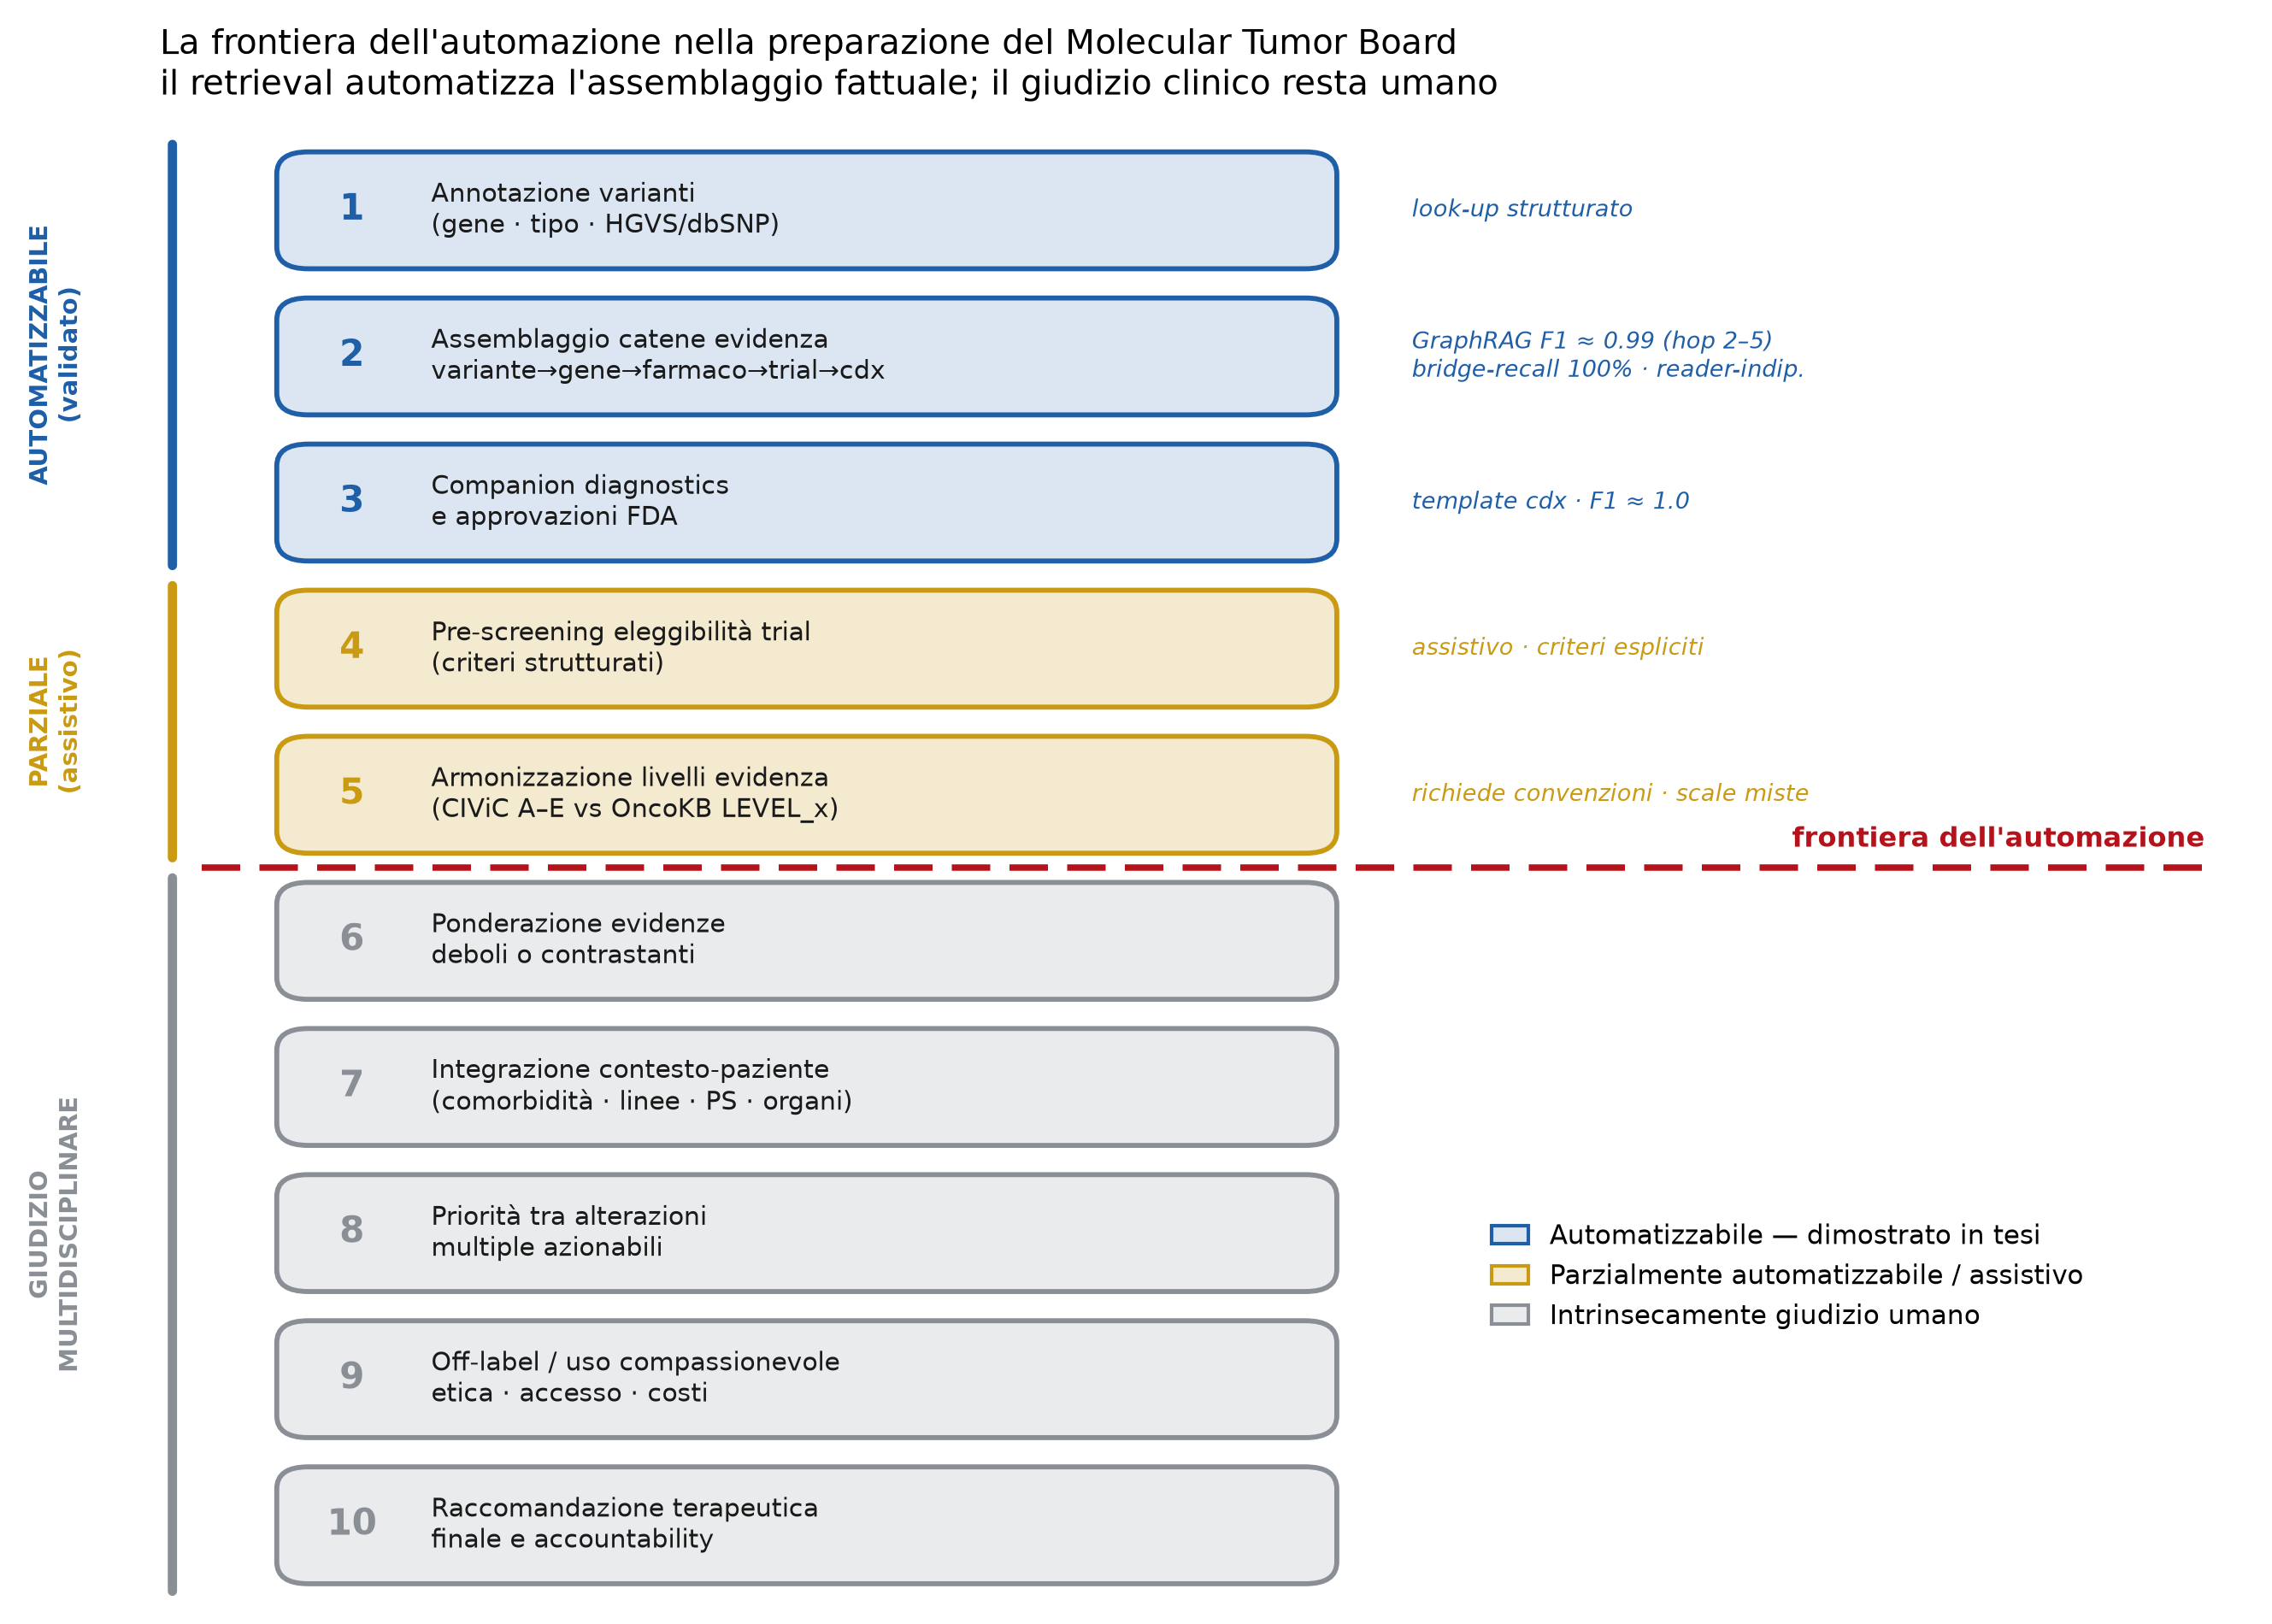
\includegraphics[width=0.98\textwidth]{fig9_automation_frontier.png}
\caption{La frontiera dell'automazione nella preparazione del Molecular
Tumor Board. I dieci stadi sono mappati in tre zone; i numeri empirici
(F1, bridge-recall) sono agganciati agli stadi che il sistema automatizza.
La linea rossa marca il confine tra recupero fattuale e giudizio clinico.}
\label{fig:frontiera}
\end{figure}

\section{Sopra la frontiera: il lavoro fattuale è delegabile}

Gli stadi 1--3 sono esattamente la parte \emph{tediosa e soggetta a errore}
della preparazione: recuperare e incrociare decine di associazioni
variante--farmaco--evidenza--trial da fonti eterogenee (CIViC, DGIdb,
ClinicalTrials.gov, FDA). È il lavoro che oggi consuma le ore di un analista
o di un biologo molecolare.

I risultati mostrano che questo lavoro è dimostrabilmente delegabile. Il
GraphRAG risolve le catene di ragionamento con \textbf{F1 $\approx$ 0,99
fino a 5 hop}, recuperando il \textbf{100\% dei fatti-ponte} necessari, e lo
fa con circa \textbf{25 volte meno contesto} del RAG testuale. Il vantaggio
non è un artefatto del particolare modello di lettura: sostituendo
completamente il reader (da \texttt{gemma3:27b} a \texttt{qwen3-coder-next},
famiglie e addestramenti diversi) la gerarchia non si muove a nessuna
profondità di hop. Ed è robusto alla riformulazione: le stesse domande
espresse in linguaggio clinico naturale non degradano la capacità del grafo
di seguire il cammino corretto.

\section{La frontiera è sicura perché il sistema la conosce}

Il punto concettualmente più importante non è l'accuratezza, ma
l'\emph{astensione}. Un sistema che automatizza il recupero fattuale in
ambito clinico è difendibile solo se sa riconoscere \emph{quando non ha una
risposta}. È qui che la struttura del grafo offre una garanzia che il RAG
testuale non può dare: quando la catena di fatti richiesta non esiste, il
GraphRAG produce un \textbf{contesto vuoto in modo deterministico}, e con un
guardrail elementare risponde ``NON DETERMINABILE'' invece di confabulare.

Sul benchmark di sicurezza il GraphRAG raggiunge il \textbf{punto ideale}:
astensione perfetta (1,00) sulle domande-trappola, zero allucinazioni, e
nessuna perdita sui controlli legittimi. In altre parole, il sistema
\textbf{restituisce l'incertezza al board umano invece di mascherarla}. È
proprio questa proprietà a tenerlo dal lato giusto della frontiera: non
invade il territorio del giudizio spacciando congetture per fatti.

\section{Sotto la frontiera: il giudizio resta umano}

Gli stadi 6--10 non contengono ``fatti da recuperare'': contengono
\emph{valutazioni da pesare}. Un'evidenza di livello D su un trial di fase I
va bilanciata contro la tossicità attesa nel paziente specifico, le linee di
terapia già fallite, l'accesso effettivo al farmaco, il performance status,
le comorbidità. Nessuno di questi elementi è nel grafo --- e non per un
limite implementativo che una versione futura potrebbe colmare, ma perché
\textbf{sono giudizi contestuali e responsabilità professionali}, non
associazioni recuperabili da una banca dati.

Gli stadi 4 e 5 stanno sulla frontiera stessa: il pre-screening di
eleggibilità e l'armonizzazione dei livelli di evidenza sono
parzialmente automatizzabili come supporto, ma richiedono convenzioni
esplicite e restano soggetti a verifica umana --- come mostra lo stesso
dataset, in cui coesistono scale di evidenza eterogenee (CIViC A--E e
OncoKB \texttt{LEVEL\_x}) che nessuna regola puramente sintattica può
riconciliare senza una decisione di merito.

\section{Conclusione}

L'automazione non sposta il confine tra macchina e clinico \emph{lungo} il
workflow MTB; lo rende \textbf{esplicito e sicuro}. La preparazione fattuale
--- assemblaggio e cross-referencing dell'evidenza molecolare --- è
largamente automatizzabile con affidabilità e, soprattutto, con astensione
deterministica sui casi senza risposta. Il giudizio multidisciplinare ---
ponderazione, contestualizzazione al paziente, priorità, responsabilità ---
resta intrinsecamente umano.

Il valore di un sistema come questo non è dunque rispondere \emph{di più},
ma sapere \emph{dove smettere di rispondere}: consegnare al Molecular Tumor
Board un dossier fattuale verificato, tracciabile fino alle fonti curate, e
insieme i suoi limiti dichiarati. È il board, non il sistema, a prendere la
decisione terapeutica --- ed è esattamente così che deve essere.

% ============================================================================
% CAPITOLO 3 — Efficienza di contesto
% ============================================================================

\chapter{Efficienza di contesto: recupero dei fatti al variare del budget}
\label{ch:efficienza-contesto}

\section{La domanda}

Il confronto principale di questa tesi fissa il budget di contesto a
\num{900} parole per tutti i sistemi. A quel budget il GraphRAG utilizza in
media circa \num{36} parole per raggiungere una recall dei fatti-gold pari a
\num{1,00}, mentre il RAG testuale ne consuma quasi \num{900} per fermarsi
molto più in basso. Un revisore può legittimamente obiettare: e se questo
divario di efficienza fosse soltanto un artefatto del budget scelto?
Concedendo al RAG testuale più contesto, il divario si chiuderebbe?

Questo capitolo risponde variando il budget su dodici livelli, da \num{100} a
\num{2400} parole, e misurando come degrada il recupero dei fatti a ciascun
livello.

\section{Metrica e metodo}

La metrica è la \textbf{recall dei fatti-gold effettivamente presenti nel
contesto} assemblato: quanta parte delle entità della risposta corretta il
sistema riesce a portare sotto gli occhi del lettore. È una quantità
\emph{deterministica} che non dipende dal modello lettore, e questo rende lo
sweep interamente offline e riproducibile senza alcuna chiave di servizio.
Per ogni livello di budget il contesto è assemblato con la stessa procedura
del sistema principale (accumulo di passaggi finché il budget è saturo). Il
GraphRAG entra come riferimento: il suo contesto è già minimo (circa \num{36}
parole) e per costruzione insensibile al budget.

\section{Risultati}

\begin{table}[H]
\centering
\caption{Recall dei fatti-gold nel contesto assemblato, al variare del budget
di contesto. Il GraphRAG è costante a \num{1,00}; BM25 e ibrido crescono
lentamente senza mai raggiungere il tetto del grafo; il denso resta molto
in basso a ogni budget.}
\label{tab:recall-budget}
\small
\begin{tabular}{r cccc}
\toprule
Budget (parole) & GraphRAG & RAG BM25 & RAG ibrido & RAG denso \\
\midrule
100  & \textbf{1,00} & 0,54 & 0,56 & 0,14 \\
150  & \textbf{1,00} & 0,58 & 0,62 & 0,18 \\
200  & \textbf{1,00} & 0,62 & 0,66 & 0,19 \\
300  & \textbf{1,00} & 0,71 & 0,73 & 0,22 \\
450  & \textbf{1,00} & 0,77 & 0,77 & 0,25 \\
600  & \textbf{1,00} & 0,80 & 0,79 & 0,27 \\
750  & \textbf{1,00} & 0,82 & 0,80 & 0,28 \\
900 (budget tesi) & \textbf{1,00} & 0,84 & 0,83 & 0,29 \\
1100 & \textbf{1,00} & 0,86 & 0,84 & 0,31 \\
1400 & \textbf{1,00} & 0,87 & 0,85 & 0,34 \\
1800 & \textbf{1,00} & 0,89 & 0,88 & 0,36 \\
2400 & \textbf{1,00} & 0,93 & 0,89 & 0,39 \\
\bottomrule
\end{tabular}
\end{table}

\begin{table}[H]
\centering
\caption{Efficienza di contesto: parole necessarie per raggiungere una data
soglia di recall dei fatti-gold. Il denso non raggiunge nessuna delle soglie
a nessun budget testato.}
\label{tab:efficienza}
\small
\begin{tabular}{c cccc}
\toprule
Soglia di recall & GraphRAG & RAG BM25 & RAG ibrido & RAG denso \\
\midrule
$\geq 60\%$ & \textbf{36} & 144 & 112 & mai \\
$\geq 70\%$ & \textbf{36} & 251 & 226 & mai \\
$\geq 80\%$ & \textbf{36} & 575 & 690 & mai \\
\bottomrule
\end{tabular}
\end{table}

\begin{figure}[H]
\centering
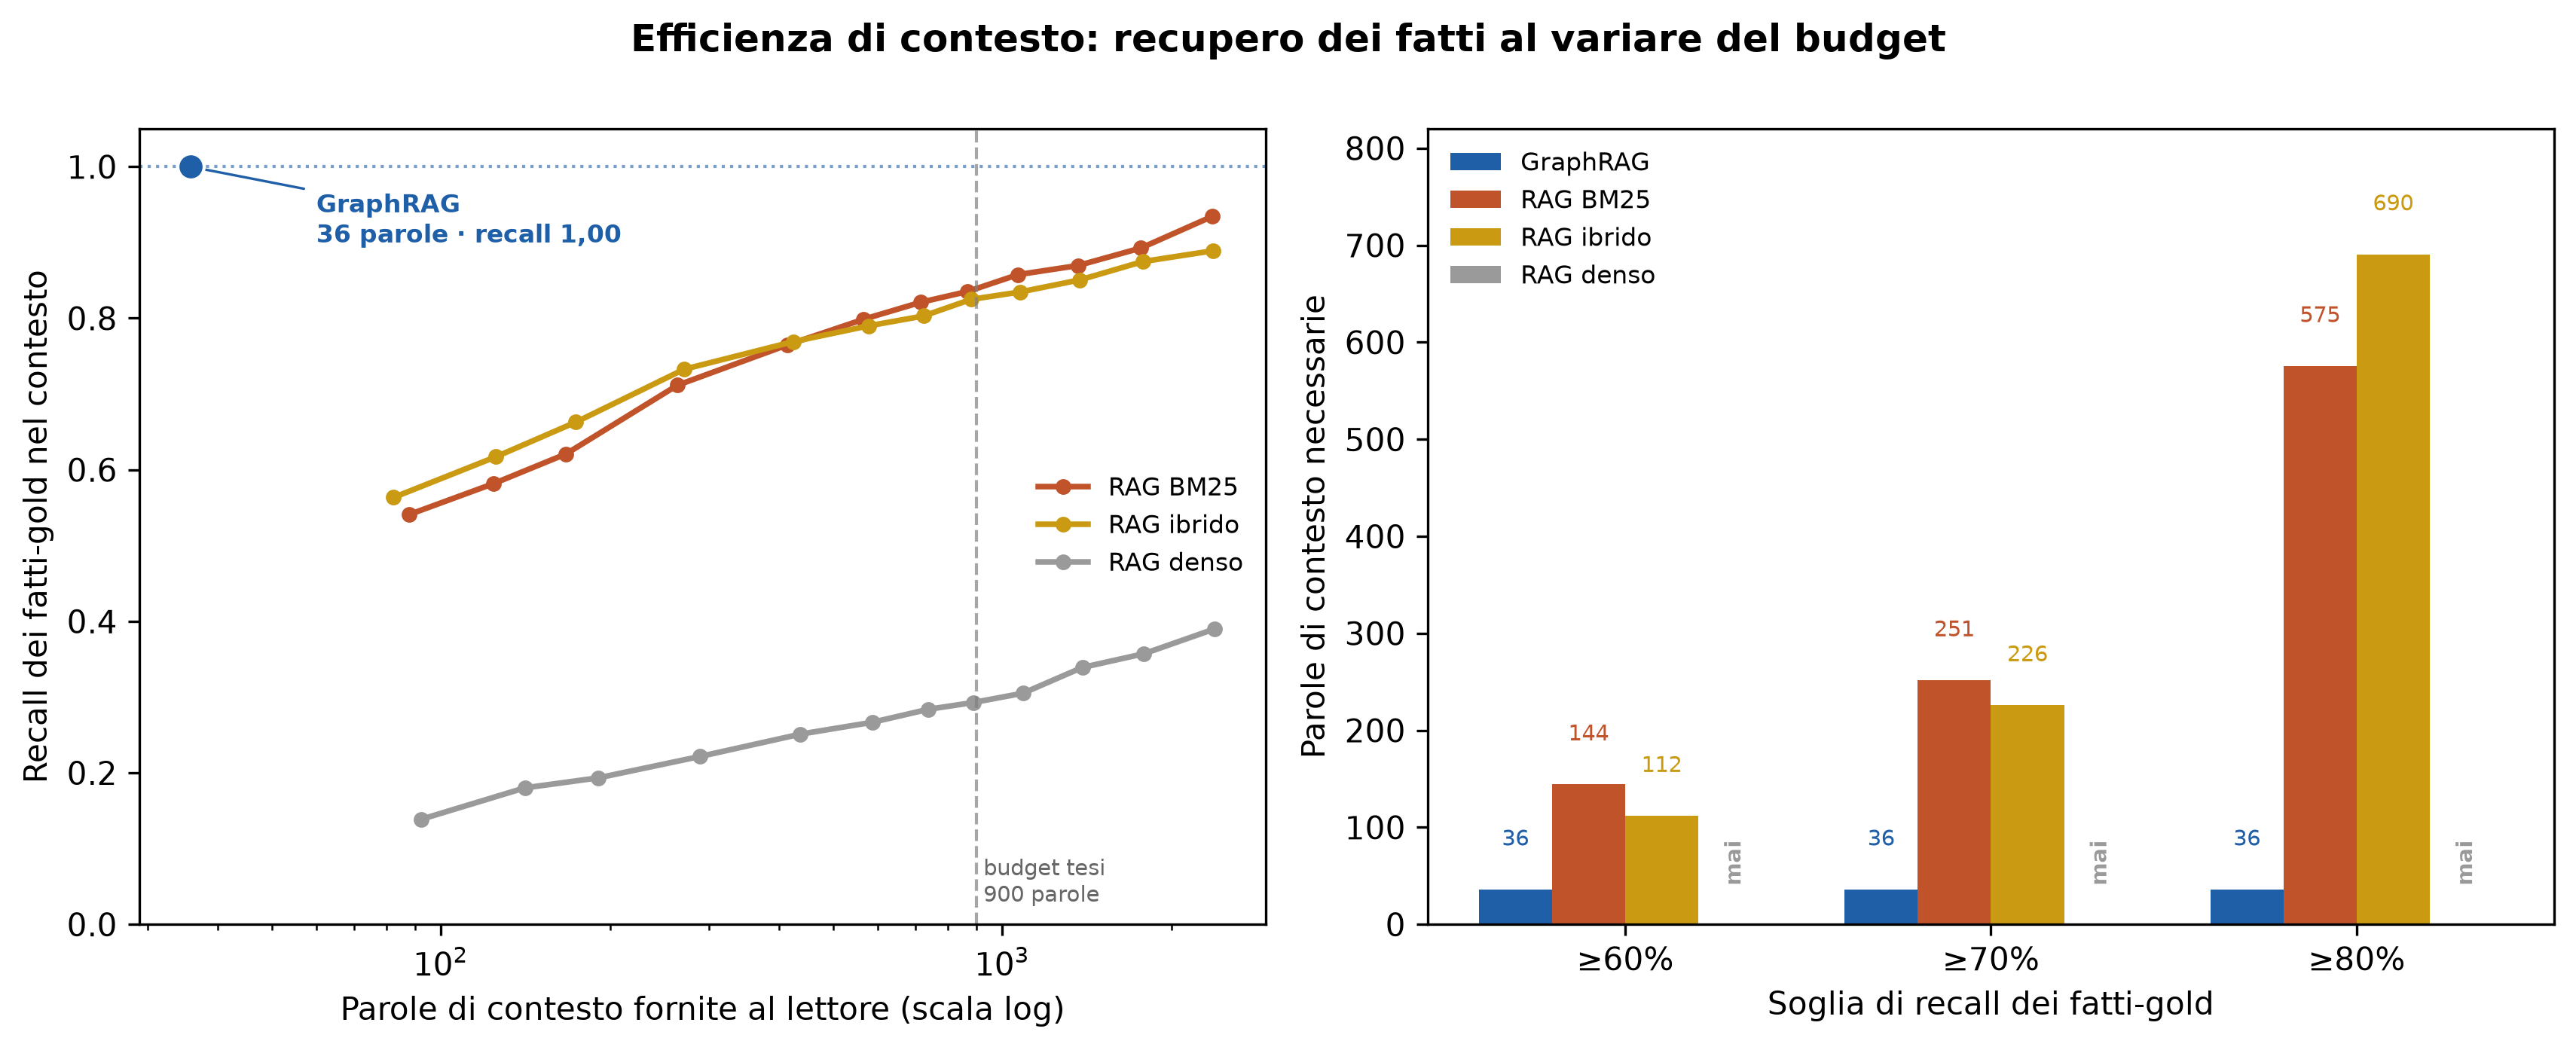
\includegraphics[width=0.98\textwidth]{fig10_context_budget.png}
\caption{Efficienza di contesto. (a) Recall dei fatti-gold in funzione delle
parole di contesto fornite al lettore (scala logaritmica): il GraphRAG è un
singolo punto in alto a sinistra (\num{36} parole, recall \num{1,00}), i RAG
testuali risalgono lentamente al crescere del contesto. (b) Parole di
contesto necessarie per raggiungere le soglie di recall del \num{60}, \num{70}
e \num{80}\%: il denso non le raggiunge mai.}
\label{fig:efficienza-contesto}
\end{figure}

\section{Interpretazione}

\textbf{Il vantaggio del GraphRAG non dipende dal budget scelto.} Anche
concedendo al RAG testuale \num{2400} parole (circa \num{2,7} volte il budget
della tesi), BM25 arriva a \num{0,93} e l'ibrido satura intorno a \num{0,89}:
nessuno dei due raggiunge il tetto del grafo (\num{1,00} con circa \num{36}
parole). Per la soglia di recall $\geq 80\%$ il GraphRAG è circa \textbf{16
volte} più efficiente di BM25 e \textbf{19 volte} più efficiente dell'ibrido.

\textbf{Il RAG denso è limitato dall'encoder, non dal contesto.} La sua
recall passa da \num{0,14} a soli \num{0,39} lungo tutto lo sweep e non
raggiunge mai neppure il \num{60}\%. Allargare il budget non lo aiuta: il
collo di bottiglia è l'encoder generico, non lo spazio di contesto. Questo
motiva, come esperimento distinto, la sostituzione con un encoder biomedico
dedicato (MedCPT, PubMedBERT, SapBERT).

\textbf{Per BM25 e ibrido il collo di bottiglia si sdoppia.} Già a \num{900}
parole la recall di retrieval (circa \num{0,83}) supera la F1 end-to-end del
lettore (circa \num{0,67} nella run principale): oltre un certo budget il
limite non è più il recupero, ma il ragionamento del lettore su un contesto
testuale lungo e rumoroso. Aggiungere parole recupera qualche fatto in più,
ma introduce anche più distrattori.

\section{Conclusione}

La curva di degrado conferma che l'efficienza di contesto del GraphRAG è una
proprietà \textbf{strutturale}, non un effetto della parametrizzazione. Il
grafo consegna al lettore esattamente i fatti-ponte richiesti in poche decine
di parole; il RAG testuale deve inondare il lettore di contesto per
avvicinarsi, senza mai raggiungere lo stesso tetto di recall. Il confronto a
\num{900} parole del capitolo principale non favorisce dunque il GraphRAG:
semmai lo penalizza, perché gli assegna un budget molto più grande di quello
che gli serve.

% ============================================================================
% CAPITOLO 4 — Baseline denso biomedico
% ============================================================================

\chapter{Baseline denso biomedico: encoder o retrieval?}
\label{ch:baseline-denso-biomedico}

\section{La domanda}

Nel confronto principale il \textbf{RAG denso} è la configurazione più
debole: la recall dei fatti-gold cresce da \num{0,14} (con \num{100} parole di
contesto) a soli \num{0,39} (con \num{2400} parole), sempre molto al di sotto
del retrieval lessicale e lontanissima dal tetto del GraphRAG (\num{1,00}).
Prima di concludere che \guillemotleft{}il retrieval denso non funziona su questa base di
conoscenza\guillemotright{} occorre isolare la causa. Il divario nasce dall'\textbf{encoder}
--- \texttt{all-MiniLM-L6-v2}, addestrato su testo generico, privo di
vocabolario biomedico --- oppure è un limite \textbf{strutturale} del dense
retrieval su un corpus fatto di fatti brevi e nomi propri (geni, farmaci,
varianti)?

Per rispondere ho sostituito l'encoder generico con encoder di
\textbf{dominio biomedico}, mantenendo identica la metrica --- recall dei
fatti-gold nel contesto assemblato, deterministica e offline --- e lo stesso
sweep di budget dello studio di efficienza di contesto.

\section{Sistemi confrontati}

Il disegno sperimentale separa due contributi spesso confusi: il
\emph{pre-training di dominio} (esporre l'encoder a testo biomedico) e il
\emph{fine-tuning per il retrieval} (addestrarlo a rendere vicine coppie
domanda--passaggio rilevanti). Per questo confronto due encoder biomedici, uno
per ciascun contributo:

\begin{table}[H]
\centering
\begin{tabularx}{\textwidth}{@{}llX@{}}
\toprule
\textbf{Sistema} & \textbf{Encoder} & \textbf{Natura} \\
\midrule
RAG denso (all-MiniLM) & \texttt{all-MiniLM-L6-v2} (384) & generico, retrieval-tuned \\
RAG denso (PubMedBERT grezzo) & \texttt{BiomedBERT} (768, mean-pool) & \textbf{solo} pre-training di dominio \\
RAG denso (PubMedBERT-MS) & \texttt{S-PubMedBert-MS-MARCO} (768) & dominio \textbf{+} fine-tuning retrieval \\
\bottomrule
\end{tabularx}
\caption{I tre encoder densi a confronto. Il PubMedBERT grezzo (masked-LM con
mean-pooling) isola l'effetto del solo dominio; \texttt{S-PubMedBert-MS-MARCO}
aggiunge il fine-tuning contrastivo su MS-MARCO.}
\end{table}

Riferimenti già misurati nello sweep: GraphRAG (\num{1,00} piatto), BM25 e
ibrido.

\section{Risultati}

\begin{table}[H]
\centering
\begin{tabular}{@{}lccc@{}}
\toprule
\textbf{Sistema} & \textbf{\num{100} parole} & \textbf{\num{900} parole} & \textbf{\num{2400} parole} \\
\midrule
\textbf{GraphRAG} & \textbf{\num{1,000}} & \textbf{\num{1,000}} & \textbf{\num{1,000}} \\
RAG BM25 & \num{0,541} & \num{0,835} & \num{0,934} \\
RAG ibrido & \num{0,563} & \num{0,825} & \num{0,889} \\
RAG denso (PubMedBERT-MS) & \num{0,369} & \textbf{\num{0,639}} & \num{0,764} \\
RAG denso (all-MiniLM) & \num{0,139} & \num{0,293} & \num{0,390} \\
RAG denso (PubMedBERT grezzo) & \num{0,017} & \num{0,144} & \num{0,244} \\
\bottomrule
\end{tabular}
\caption{Recall dei fatti-gold nel contesto a tre budget rappresentativi.}
\end{table}

\begin{table}[H]
\centering
\begin{tabular}{@{}lccc@{}}
\toprule
\textbf{Sistema} & \textbf{$\geq$\SI{60}{\percent}} & \textbf{$\geq$\SI{70}{\percent}} & \textbf{$\geq$\SI{80}{\percent}} \\
\midrule
GraphRAG & \num{36} & \num{36} & \num{36} \\
RAG BM25 & \num{144} & \num{251} & \num{575} \\
RAG ibrido & \num{112} & \num{226} & \num{690} \\
RAG denso (PubMedBERT-MS) & \num{669} & \num{1543} & mai \\
RAG denso (all-MiniLM) & mai & mai & mai \\
RAG denso (PubMedBERT grezzo) & mai & mai & mai \\
\bottomrule
\end{tabular}
\caption{Parole di contesto necessarie per raggiungere una soglia di recall.
\guillemotleft{}mai\guillemotright{} indica che la soglia non viene raggiunta neppure a \num{2400} parole.}
\end{table}

\begin{figure}[H]
\centering
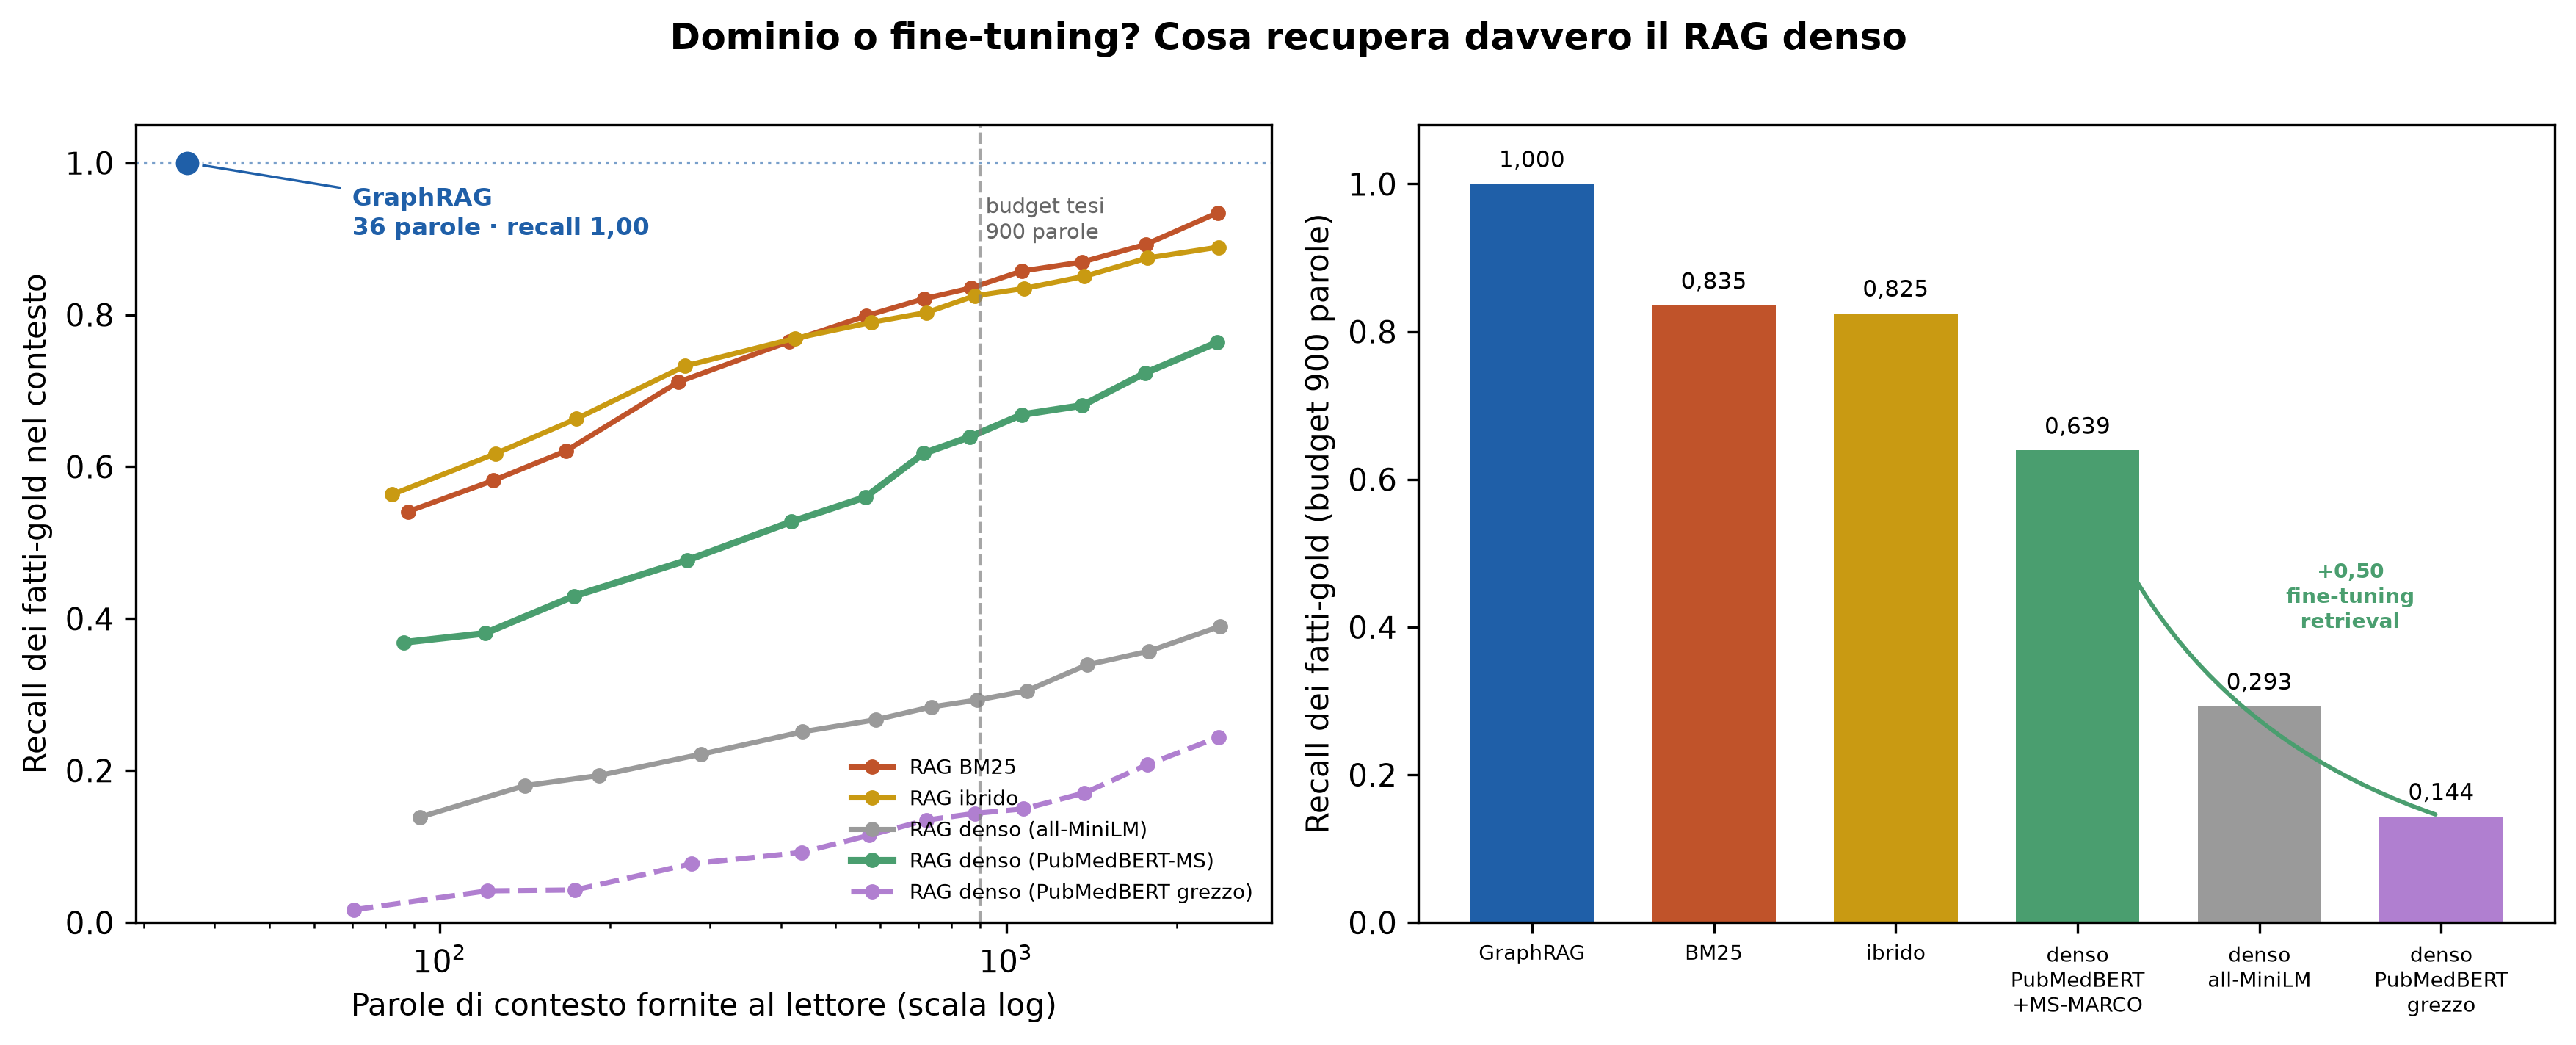
\includegraphics[width=\textwidth]{fig11_biomedical_dense.png}
\caption{\textbf{(a)} Recall dei fatti-gold in funzione delle parole di
contesto (scala logaritmica): l'encoder biomedico retrieval-tuned (verde) si
stacca nettamente dal generico (grigio), mentre il PubMedBERT grezzo
(tratteggiato viola) resta il più basso. \textbf{(b)} Recall a budget \num{900}
parole: il salto da PubMedBERT grezzo (\num{0,144}) a PubMedBERT-MS
(\num{0,639}) misura l'effetto del solo fine-tuning per il retrieval.}
\end{figure}

\section{Tre conclusioni}

\textbf{1. L'encoder biomedico recupera gran parte del divario --- ma non
tutto.} Passando da \texttt{all-MiniLM} a \texttt{S-PubMedBert-MS-MARCO} la
recall a budget \num{900} più che raddoppia: \num{0,293} $\rightarrow$
\num{0,639}. Il denso biomedico supera le soglie del \SI{60}{\percent} (a
\num{669} parole) e del \SI{70}{\percent} (a \num{1543} parole), che l'encoder
generico non raggiunge \emph{mai}. Il divario del RAG denso era dunque in
larga parte un \textbf{artefatto dell'encoder}, non un limite assoluto del
metodo.

\textbf{2. Non è il vocabolario biomedico a contare, ma il fine-tuning per il
retrieval.} Il controllo decisivo è il PubMedBERT \textbf{grezzo}: solo
masked-LM su testo biomedico, mean-pooling, nessun obiettivo contrastivo. La
sua recall a budget \num{900} è \num{0,144}, \textbf{peggiore} persino
dell'encoder generico (\num{0,293}). Il pre-training di dominio da solo produce
embedding inadatti al retrieval; è il fine-tuning su coppie domanda--passaggio
(MS-MARCO) a spostare la recall da \num{0,144} a \num{0,639}. Per il retrieval
conta \textbf{come} l'encoder è stato addestrato, non solo \textbf{su quale}
dominio.

\textbf{3. Anche il miglior encoder denso resta sotto il lessicale e lontano
dal grafo.} A budget \num{900} il denso biomedico (\num{0,639}) non raggiunge
né BM25 (\num{0,835}) né l'ibrido (\num{0,825}); e anche a \num{2400} parole
(\num{0,764}) non tocca il tetto del grafo (\num{1,00}), che il GraphRAG
raggiunge con \num{36} parole. Su una base di conoscenza fatta di nomi propri e
fatti brevi --- dove conta la corrispondenza esatta di un simbolo genico o di
un nome di farmaco --- il retrieval lessicale e quello strutturato del grafo
restano più adatti della similarità densa, per quanto specializzata.

\section{Implicazione per la tesi}

Questo esperimento chiude una possibile obiezione al confronto principale
(\guillemotleft{}il RAG denso perde solo perché usa un encoder generico\guillemotright{}). La risposta è
articolata: un encoder biomedico \emph{retrieval-tuned} recupera buona parte
del divario e va adottato come baseline denso corretto; tuttavia neppure quel
sistema raggiunge la recall del retrieval lessicale, né la compattezza e la
completezza del GraphRAG. Il vantaggio del grafo --- recall \num{1,00} con
\num{36} parole di contesto --- non è replicabile aumentando la dimensionalità
o la specializzazione dell'encoder denso, perché deriva dal \textbf{modo} in
cui i fatti sono collegati, non dalla loro rappresentazione vettoriale.

% ============================================================================
% CAPITOLO 5 — Scaling della profondità dei salti
% ============================================================================

\chapter{Scaling della profondità dei salti}
\label{ch:profondita-salti}

\section{Domanda sperimentale}

Fino a che punto la struttura del grafo continua a proteggere il recupero quando la catena
di ragionamento clinico si allunga? Gli esperimenti precedenti hanno lavorato su domande a
2--5 salti. Qui portiamo la profondità fino a \textbf{8 salti} e misuriamo due grandezze
distinte, entrambe in modo deterministico e offline (router = oracolo, nessun modello
linguistico nel ciclo di misura):

\begin{enumerate}
  \item \textbf{Recall del fatto terminale} --- il nome dell'entità-obiettivo finale compare
        nel contesto recuperato?
  \item \textbf{Chain-recall (completezza della catena)} --- quale frazione dei nomi-ponte
        intermedi compare nel contesto?
\end{enumerate}

La seconda metrica è il cuore di questo esperimento: una risposta a molti salti è utile non
solo se contiene il fatto finale, ma se contiene \emph{tutti gli anelli} che lo giustificano.

\section{Disegno: una spina tipizzata, lo stesso gene ad ogni profondità}

Il rischio metodologico in un esperimento di profondità è confondere la profondità con la
scelta del sotto-grafo. Lo evitiamo con una \textbf{spina tipizzata unica}:

\begin{quote}\itshape
Gene $\rightarrow$ Variant $\rightarrow$ MolecularProfile $\rightarrow$ Evidence
$\rightarrow$ Drug $\rightarrow$ CompanionDiagnostic $\rightarrow$ Gene$'$
$\rightarrow$ Variant$'$ $\rightarrow$ MolecularProfile$'$
\end{quote}

Ogni gene-ancora che possiede un \textbf{cammino canonico completo} a profondità 8
(\num{91} geni, selezionati fra \num{1437}; visita in profondità deterministica con
successori mescolati dal seme \texttt{20240517}) viene troncato a profondità crescenti.
Poiché \textbf{lo stesso gene} genera la domanda ad ogni profondità, la profondità resta
l'unica variabile manipolata.

La profondità~3 ha come terminale un nodo \textsf{Evidence}, che nel grafo \textbf{non ha
attributo \texttt{name}}: non è nominabile in un test testuale, quindi è esclusa. Le
profondità usate sono \textbf{1, 2, 4, 5, 6, 7, 8}, per un totale di \num{637} domande
(\num{91} ancore $\times$ 7 profondità).

\section{La covariata onesta: quanti passaggi separati servono}

Prima dei risultati documentiamo il meccanismo che spiega \emph{perché} la
profondità incide sul recupero testuale. Per ciascun cammino canonico si può
contare quanti \textbf{passaggi distinti} del corpus servono per testimoniare
l'intera catena: un passaggio ``testimonia'' un salto se il suo testo contiene
i nomi di entrambi gli estremi dell'arco.

Finché la catena è corta --- fino a circa 4 salti --- la mediana del numero
di passaggi necessari è \textbf{1}: l'intera catena vive dentro un singolo
passaggio ricco, perché il corpus è \emph{evidence-centric} e un passaggio
raggruppa gene, variante, profilo molecolare, evidenza e farmaco. Questo
spiega perché, a profondità basse, anche il RAG testuale riesce a recuperare
buona parte dei fatti necessari: gli basta trovare il passaggio giusto e
quello contiene tutto.

Da profondità~5 in poi la situazione cambia in modo qualitativo: la catena
smette di vivere in un unico passaggio. La mediana dei passaggi necessari
sale a \textbf{2} (profondità~5), poi a \textbf{3} (profondità~7) e a
\textbf{4} (profondità~8). Il RAG testuale deve quindi \textbf{recuperare e
unire passaggi separati}, ciascuno dei quali copre solo un segmento della
catena. Ed è esattamente a questa transizione che ci aspettiamo --- e
osserviamo --- il crollo del recupero testuale: la probabilità di recuperare
\emph{tutti} i segmenti necessari diminuisce moltiplicativamente con il
numero di passaggi da assemblare.

\section{Risultati}

\begin{figure}[H]
  \centering
  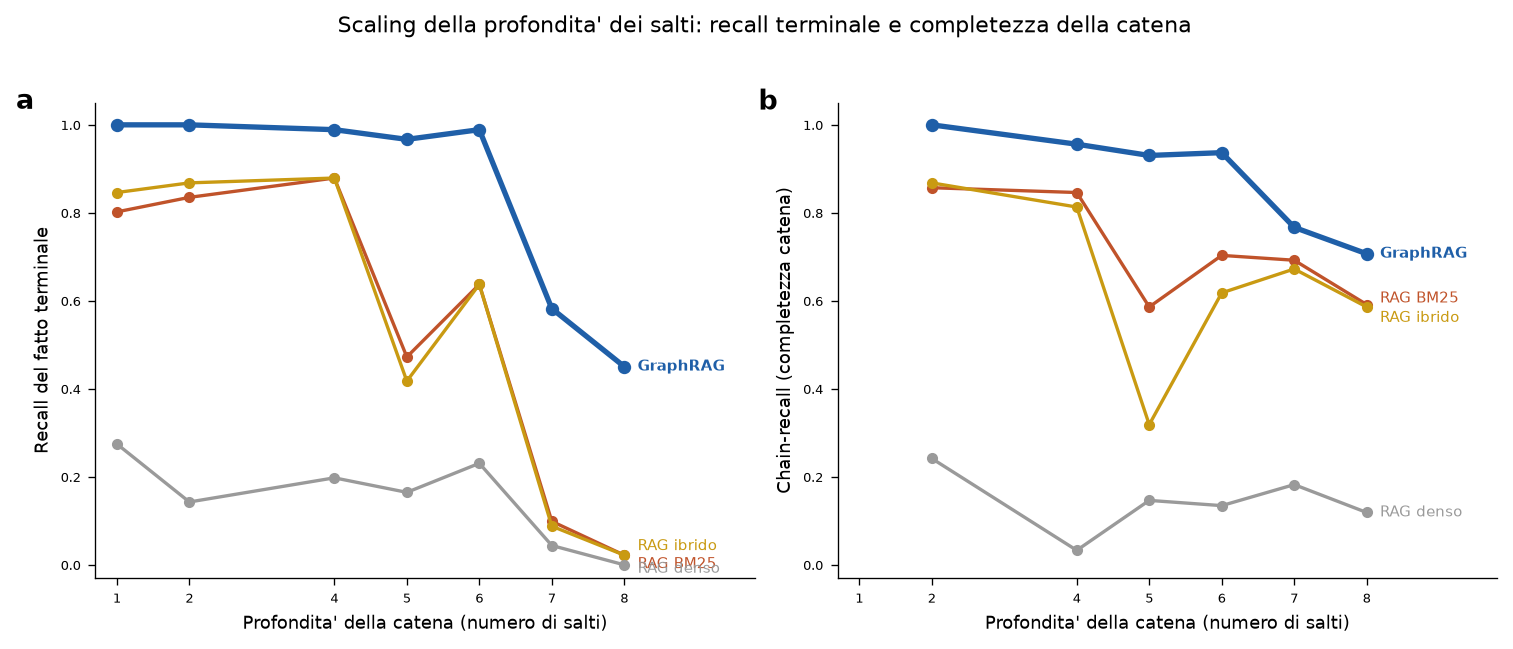
\includegraphics[width=\textwidth]{fig13_profondita_salti.png}
  \caption{Scaling della profondità dei salti. (a)~Recall del fatto terminale vs profondità.
  (b)~Chain-recall (completezza della catena) vs profondità. \gr{} (blu) è la linea focale.}
  \label{fig:fig13}
\end{figure}

\subsection{Recall del fatto terminale}

\begin{table}[H]
  \centering
  \sisetup{table-format=1.3}
  \begin{tabular}{r S S S S}
    \toprule
    Profondità & {\gr} & {RAG BM25} & {RAG ibrido} & {RAG denso} \\
    \midrule
    1 & 1.000 & 0.802 & 0.846 & 0.275 \\
    2 & 1.000 & 0.835 & 0.868 & 0.143 \\
    4 & 0.989 & 0.879 & 0.879 & 0.198 \\
    5 & 0.967 & 0.473 & 0.418 & 0.165 \\
    6 & 0.989 & 0.637 & 0.637 & 0.231 \\
    7 & 0.582 & 0.099 & 0.088 & 0.044 \\
    8 & 0.451 & 0.022 & 0.022 & 0.000 \\
    \bottomrule
  \end{tabular}
  \caption{Recall del fatto terminale per sistema e profondità.}
\end{table}

\gr{} \textbf{domina ad ogni profondità}. Il salto~5 (Farmaco~$\rightarrow$~Test
diagnostico) è un vero scoglio per il RAG: la recall di BM25 crolla da \num{0.879} a
\num{0.473} perché il farmaco e il suo test di accompagnamento \textbf{non sono più
co-menzionati nello stesso passaggio}. \gr{}, che attraversa l'arco
\textsf{HAS\_COMPANION\_DIAGNOSTIC} esplicitamente, resta a \num{0.967}.

Il calo di \gr{} a profondità 7--8 è un \textbf{confondimento di fan-out documentato, non un
guasto}. Il settimo salto è un secondo \textsf{HAS\_VARIANT}: il gene raggiunto può
ramificare in decine di varianti. Per ABCB1 la profondità~8 genera \num{162} cammini; sotto
il budget di \num{900} parole solo circa 17 vengono serializzati, quindi lo \emph{specifico}
terminale canonico compete con i suoi fratelli e non sempre entra nel contesto. È recupero
limitato dal budget su un ventaglio combinatorio --- la stessa pressione che la covariata di
fan-out anticipa.

\subsection{Chain-recall / completezza della catena}

\begin{table}[H]
  \centering
  \sisetup{table-format=1.3}
  \begin{tabular}{r S S S S}
    \toprule
    Profondità & {\gr} & {RAG BM25} & {RAG ibrido} & {RAG denso} \\
    \midrule
    2 & 1.000 & 0.857 & 0.868 & 0.242 \\
    4 & 0.956 & 0.846 & 0.813 & 0.033 \\
    5 & 0.930 & 0.586 & 0.319 & 0.147 \\
    6 & 0.937 & 0.703 & 0.618 & 0.135 \\
    7 & 0.767 & 0.692 & 0.673 & 0.182 \\
    8 & 0.707 & 0.592 & 0.586 & 0.119 \\
    \bottomrule
  \end{tabular}
  \caption{Chain-recall (frazione dei nomi-ponte presenti nel contesto) per sistema e
  profondità. La profondità~1 non ha ponti intermedi.}
\end{table}

Qui emerge la proprietà strutturale di \gr{}. Ogni cammino serializzato è \textbf{internamente
completo per costruzione} --- nomina tutti i nodi-ponte lungo la spina --- quindi la
chain-recall \textbf{degrada con grazia} (\num{1.000}~$\rightarrow$~\num{0.707}) invece di
crollare. Il RAG denso, che deve coprire ogni salto in modo indipendente, resta
\textbf{sotto \num{0.20}} a ogni profondità: la probabilità che un singolo recupero copra
\emph{tutti} gli anelli decade moltiplicativamente. BM25 e ibrido tengono meglio del denso
ma restano circa \num{0.12}--\num{0.15} sotto \gr{} per tutta la coda.

Si noti che a profondità 7--8 la chain-recall di \gr{} (\num{0.767} / \num{0.707}) è
\textbf{molto più alta} della sua recall terminale (\num{0.582} / \num{0.451}): anche quando
il budget espelle lo specifico terminale, gli anelli intermedi della catena restano in gran
parte nel contesto. La struttura preserva il \emph{ragionamento} anche dove il ventaglio
combinatorio mette sotto pressione la singola risposta finale.

\section{Conclusioni}

\begin{enumerate}
  \item \textbf{La struttura protegge il recupero profondo.} Su terminale e catena, \gr{} è
        superiore ad ogni profondità; il divario si allarga proprio dove la catena smette di
        vivere in un unico passaggio (profondità $\geq 5$).
  \item \textbf{La completezza della catena è la metrica che separa i paradigmi.} \gr{}
        degrada con grazia perché ogni cammino è completo per costruzione; il RAG denso
        collassa perché deve coprire ogni salto in modo indipendente.
  \item \textbf{Il limite di \gr{} è il budget, non la connettività.} Il calo terminale a
        profondità 7--8 è ventaglio combinatorio sotto un budget fisso di \num{900} parole
        --- un limite di \emph{impaginazione}, non di \emph{raggiungibilità}: la connettività
        del grafo garantisce che il terminale sia sempre a distanza finita; è la
        serializzazione a doverlo scegliere fra molti fratelli.
\end{enumerate}

% ============================================================================
% APPENDICE — Il test di McNemar
% ============================================================================

\appendix
\chapter{Il test di McNemar: significato e ruolo negli esperimenti}
\label{app:mcnemar}

\section{Che cos'è il test di McNemar}

Il test di McNemar è un test statistico non parametrico che serve a
confrontare le prestazioni di \textbf{due classificatori sullo stesso insieme
di dati}. A differenza di un semplice confronto di percentuali, il test
tiene conto del fatto che le osservazioni sono \emph{appaiate}: ogni domanda
è stata sottoposta a entrambi i sistemi, e ci interessa sapere se le
differenze osservate sono sistematiche o frutto del caso.

\section{Come funziona}

Il punto di partenza è una tabella di contingenza $2 \times 2$ che
classifica ogni domanda in base all'esito dei due sistemi:

\begin{table}[H]
\centering
\begin{tabular}{lcc}
\toprule
 & \textbf{Sistema B corretto} & \textbf{Sistema B sbagliato} \\
\midrule
\textbf{Sistema A corretto} & $a$ (entrambi corretti)  & $b$ (solo A corretto) \\
\textbf{Sistema A sbagliato} & $c$ (solo B corretto) & $d$ (entrambi sbagliati) \\
\bottomrule
\end{tabular}
\caption{Tabella di contingenza per il test di McNemar. Le celle $b$ e $c$
(i casi ``discordanti'') sono le uniche informative.}
\end{table}

Le celle $a$ e $d$ --- le domande su cui i due sistemi concordano --- non
contribuiscono al test: se entrambi rispondono bene o entrambi sbagliano,
non c'è evidenza di una differenza. Tutta l'informazione sta nelle celle
\textbf{discordanti} $b$ e $c$: le domande su cui un sistema risponde
correttamente e l'altro no.

L'ipotesi nulla è che i due sistemi abbiano la stessa probabilità di
rispondere correttamente, il che implica $b = c$ in valore atteso. La
statistica del test è:
\[
\chi^2_{\text{McNemar}} = \frac{(b - c)^2}{b + c}
\]
che segue approssimativamente una distribuzione $\chi^2$ con 1 grado di
libertà. Un valore grande indica che i casi discordanti pendono
sistematicamente a favore di uno dei due sistemi.

\section{Perché è appropriato per questi esperimenti}

Nel confronto GraphRAG contro RAG testuale, ogni domanda del benchmark è
stata sottoposta a tutti i sistemi nelle stesse condizioni. Le risposte sono
binarie (corretta / sbagliata) e appaiate per domanda: esattamente la
situazione per cui il test di McNemar è progettato.

Alternative come il test $t$ o il test $\chi^2$ di indipendenza sarebbero
inappropriate: il primo assume normalità e osservazioni continue; il secondo
non tiene conto dell'appaiamento e tratterebbe i risultati come se venissero
da campioni indipendenti, perdendo potenza statistica e rischiando
conclusioni errate.

\section{Come è stato usato nella tesi}

Nel Capitolo~\ref{ch:graphrag-vs-rag}, il test di McNemar è stato applicato
per verificare che il vantaggio del GraphRAG rispetto a ciascuno dei tre
sistemi RAG testuali non fosse un artefatto del campione di domande. I
risultati sono netti:

\begin{itemize}
  \item \textbf{GraphRAG vs RAG BM25}: il GraphRAG risponde correttamente
        dove BM25 sbaglia in $b = 50$ domande; il contrario accade in
        $c = 1$ sola domanda. $p = 4{,}6 \times 10^{-14}$.
  \item \textbf{GraphRAG vs RAG ibrido}: $b = 54$, $c = 1$.
        $p = 3{,}1 \times 10^{-15}$.
  \item \textbf{GraphRAG vs RAG denso}: $b = 142$, $c = 0$.
        $p = 3{,}6 \times 10^{-43}$.
\end{itemize}

In tutti e tre i casi l'asimmetria è schiacciante e i valori $p$ sono
inferiori a qualsiasi soglia convenzionale ($0{,}05$, $0{,}01$, $0{,}001$).
Questo significa che la superiorità del GraphRAG non è spiegabile dal caso:
è una proprietà sistematica del metodo di recupero, non una fluttuazione
statistica legata alle specifiche domande del benchmark.

\section{Il ruolo nel quadro complessivo}

Il test di McNemar svolge una funzione precisa nella catena argomentativa
della tesi: trasforma un'osservazione descrittiva (``il GraphRAG ha un F1
più alto'') in un'\textbf{affermazione statisticamente fondata} (``il
divario è sistematico e non attribuibile al caso''). Senza questo
passaggio, un critico potrebbe obiettare che le 169 domande del benchmark
siano un campione sfortunato; con il test, questa obiezione è
quantitativamente esclusa.

\end{document}
